\section{Ripasso}

Si ricordano le definizioni di algoritmo e problema computazionale astratto:

\begin{definition}[Algoritmo]\label{def:alg}
    Un algoritmo è una procedura computazionale finita (terminante) e deterministica, specificata come una sequenza di passi elementari (istruzioni) estratte da un insieme standard associato a un modello computazionale (astrazione di un computer) che trasforma in maniera univoca un ingresso in un uscita.
\end{definition}


\begin{definition}[Problema computazionale]\label{def:probcomp}
    Un problema computazionale $\bpi{}$ è una relazione tra un insieme di istanze $\bi{}$ e un insieme di soluzioni $\bs{}$: $\bpi{} \subseteq \bi{} \times \bs{}$
    \\
    Un problema computazionale definisce la specifica astratta. % ma de che?
\end{definition}

Note:
% \begin{itemize}[noitemsep,topsep=0pt,parsep=0pt,partopsep=0pt]
\begin{itemize}[noitemsep,parsep=0pt,partopsep=0pt,topsep=0pt]
    \item le seguenti notazioni sono usate in maniera equivalente: $i_1 \bpi{} s_1 \iff (i_1 , s_1 ) \in \bpi{}$
    \item la relazione non è univoca, ad un'istanza possono essere associate più soluzioni
    \item nella specifica astratta si assume esistano le soluzioni per ogni istanza:\\
        $\forall i \in \bi{},\exists s \in \bs{} | i \bpi{} s$
\end{itemize}

Un algoritmo $A_{\bpi{}}$ è un algoritmo per $\bpi{}$, ossia risolve $\bpi{}$ se, quando i suoi ingressi sono elementi di $\bi{}$, le sue uscite sono gli elementi di $\bs{}$ in relazione all'ingresso, formalmente:
$$ A: \bi{} \to \bs{} \quad \textrm{e} \quad A(i)=s \iff i \, \bpi{} \, s $$

\section{Categorie di problemi}
I problemi computazionali si possono dividere in quattro categorie:

\subsubsection{Polinomiali}
Problemi $\bpi{}$ che ammettono algoritmi di risoluzione polinomiale, che si possono considerare ``facili''. Si trova una certa evidenza
% epistemologica
che i gradi in generale sono bassi, e si può considerare un problema polinomiale come trattabile.

\subsubsection{Con limite inferiore esponenziale}
Problemi $\bpi{}$ per cui si può provare che la complessità di ogni algoritmo che li risolve è esponenziale.
\begin{equation*}
    \forall A_{\bpi{}} \; \exists \, c > 1 : T_{A_{\bpi{}}} \left( n \right) = \Omega \left( c^{n} \right)
    % \label{}
\end{equation*}
I problemi per cui si riesce a dimostrare questa proprietà sono però molto pochi, in genere problemi artificiali legati ai linguaggi.

\subsubsection{Problemi che non ammettono algoritmi di risoluzione}
Ricordiamo che un algoritmo è una procedura \emph{terminante}. Per esempio l'\emph{halting problem}, si definisce come:
\begin{equation*}
    \bi{}_{H} = \left\{ \langle MT,x \rangle \right\}
    \quad
    \bs{}_{H} = \left\{ \texttt{Sì, No} \right\}
\end{equation*}
Il problema della fermata risponde \texttt{Sì} se, dati in input una macchina di Turing e un input, la computazione termina.
\begin{equation*}
    i = 
    \langle
    MT, x
    \rangle
    \:
    \bpi
    \:
    s = 
    \begin{cases}
        \texttt{Sì} & \text{ se $MT(x)$ termina} \\
        \texttt{No} & \text{ altrimenti}
    \end{cases}
\end{equation*}
La difficoltà di questo problema è dovuta alla richiesta che l'eventuale algoritmo solutore debba valere per \emph{tutti} gli input.
Molto informalmente, dato un programma $f$ che decide se le computazioni terminano, si può sempre trovare un programma patologico $g$ che, passato a $f$ insieme ad un input $x$, fa poi per quell'input l'opposto di quello che $f$ predice.
% \begin{equation*}
    % g(x) \ne f(g,x)
% \end{equation*}

\subsubsection{Problemi intrattabili}

Sono problemi per cui non esiste né un algoritmo $A_{\bpi{}}$ che li risolva, e neppure un \emph{lower bound} esponenziale.
Tuttavia c'è forte evidenza che il \emph{lower bound} esista, infatti si può provare che tutti i problemi in questa classe sono equivalenti, e questa proprietà di chiusura spinge verso la loro difficoltà.

\section{Problemi decisionali}
% pag 4.2

\subsection{Problemi di ottimizzazione}
% pag 5

In un problema di ottimizzazione, si definisce una funzione di costo associato ad una soluzione:
\begin{equation*}
    c : \bs{} \to \mathbb{R}
\end{equation*}
e, dato l'insieme di soluzioni ammissibili associate ad un'istanza
\begin{equation*}
    \bs{} (i) = \left\{ s \in \bs{} : i \, \bpi{} \, s \right\}
\end{equation*}
si vuole individuare la soluzione di costo massimo (o minimo)
\begin{equation*}
    s_{i}^{*} = \argmax \left\{ c(s) : s \in \bs{} (i) \right\}
\end{equation*}

\subsection{Problemi decisionali}
% pag 4.2

Per definire problemi e complessità degli algoritmi in modo rigoroso è necessario standardizzare i problemi computazionali.

Un problema decisionale presenta un insieme delle soluzioni ridotto a due elementi, ed associa ad un'istanza generica una risposta (positiva o negativa) ad una domanda sull'istanza.
\begin{equation*}
    \bpi{}_{D} : \bi{} \to \left\{ \texttt{Sì, No} \right\}
\end{equation*}

\subsubsection{\emph{Shortest Unweighted Path}}
% pag 4.5
% Il problema è definito sull'istanza $\langle G=(V,E), s, t \rangle$, dove $V \subseteq \mathbb{N}$ finito (i nodi sono identificati con numeri naturali), $E \subseteq V \times V$ (gli archi sono coppie ordinate di vertici), $s, t \in V$. L'insieme delle soluzioni è $\mathbb{N}^*$, e una soluzione generica è $s=<v_1, \dots, v_k$, dove $v_i \in V, v_1=s, v_k=t$ e $\left( v_i, v_{i+1} \right) \in E, 1 \leq i < k$.
La restrizione ad un insieme binario di soluzioni non comporta una perdita di generalità, per esempio, si consideri il problema di trovare un cammino minimo tra due nodi in un grafo:
\begin{align*}
    \texttt{istanza:} \quad & \langle G=(V,E), s, t \rangle \\
    \text{dove} \quad & V \subseteq \mathbb{N} \quad \text{finito (i nodi sono identificati con numeri naturali)} \\
    & E \subseteq V \times V \quad \text{(gli archi sono coppie ordinate di vertici)} \\
    & s, t \in V \\
    \texttt{soluzioni:} \quad & s=\langle v_1, \dots, v_k \rangle \in \mathbb{N}^* \\
    i \, \bpi{} s \text{ se } \quad & 
    % \text{dove} \quad &
    v_i \in V \\
    & v_1=s, \: v_k=t \\
    & \left( v_i, v_{i+1} \right) \in E, 1 \leq i < k \\
    i \, \bpi{} \, \varepsilon \text{ se } \quad & \text{non esiste cammino tra $s$ e $t$ in $G$} \\
    \texttt{costo:} \quad & c\left( \langle  v_1, \ldots, v_k  \rangle \right) = k - 1 \\
    & c( \varepsilon ) = \infty \\
    \intertext{A questo problema di ottimizzazione si può associare un problema decisionale, arricchendo l'istanza con un limite superiore alla lunghezza del cammino}
    \texttt{istanza:} \quad & \langle G=(V,E), s, t, k \rangle \\
    \texttt{domanda:} \quad & \text{esiste un cammino tra $s$ e $t$ in $G$, di lunghezza $\leq k$?} \\
\end{align*}
Avendo un algoritmo $A_{KUP}$ che risolva il problema decisionale, si può costruire facilmente un algoritmo che risolva $SUP$, usando $KUP$ come subroutine; l'algoritmo termina, perché si stanno cercando cammini semplici, quindi di lunghezza massima pari al numero di nodi meno uno.
\begin{algorithm}[H]
\caption{Shortest Unweighted Path}\label{alg:sup}
\begin{algorithmic}[1]
    \Procedure{$A_{SUP}$}{$\langle G=(V,E), s, t \rangle$}
        \State $m \gets |V|$
        \For{$k \gets 0 $ to $ m-1 $ }
        \If{\Call{$A_{KUP}$}{$\langle G=(V,E), s, t, k \rangle$} = \texttt{Sì}}
                \State return $k$
            \EndIf
        \EndFor
        \State return $\infty$
    \EndProcedure
\end{algorithmic}
\end{algorithm}
\noindent
Per quanto riguarda la complessità, si possono considerare le due istanze come di taglia paragonabile
\begin{equation*}
    |\langle G, s, t, k \rangle| = \Theta \left( |\langle G, s, t \rangle| \right)
\end{equation*}
e assumendo $KUP$ polinomiale
\begin{equation*}
    T_{KUP} = O \left( |\langle G, s, t, k \rangle|^{h} \right)
\end{equation*}
e considerando che il numero di archi è limitato dalla taglia dell'istanza
\begin{equation}
    m = O \left( |\langle G, s, t \rangle| \right)
    \label{eq:tagliamgst}
\end{equation}
si ottiene che
\begin{align*}
    T_{SUP} \left( |\langle G, s, t \rangle| \right) &= O \left( |\langle G, s, t \rangle||\langle G, s, t \rangle|^{h} \right) \\
    &= O \left( |\langle G, s, t \rangle|^{h+1} \right)
\end{align*}
per cui se si riesce a risolvere il problema decisionale si può risolvere anche il problema di ottimizzazione.

Per ESERCIZIO, si scriva un algoritmo che ritorni anche il cammino minimo. Si suggerisce, dopo aver identificato $k$, di rimuovere archi per identificare quali siano quelli necessari per il cammino cercato. La complessità può risultare di due gradi superiore a quella di $KUP$.

\section{Codifica delle istanze}
% pag 6.7
Un problema astratto generico è definito quindi come
\begin{equation*}
    \bpi{}_{A} : \bi{} \to \left\{ \texttt{Sì, No} \right\}
\end{equation*}
Come si evidenzia nell'equazione \ref{eq:tagliamgst}, c'è un forte legame tra taglia dell'istanza e complessità dell'algoritmo. Va quindi definito precisamente il concetto di codifica di un'istanza.
\begin{definition}[\emph{Encoding} (codifica)]\label{def:codifica}
L'\emph{encoding} è una funzione invertibile (iniettiva)
\begin{equation*}
    e : \bi{} \to \setzo{*}
\end{equation*}
che mappa istanze in stringhe finite (quindi considera istanze numerabili, che è ragionevole). La notazione completa è $e_{\bi{}}$ per indicare che la codifica è legata ad un preciso insieme di istanze, ma il pedice viene omesso per leggibilità.
\end{definition}

Il problema astratto viene mappato nel problema concreto
\begin{equation*}
    \bpi{}_{C} : \setzo{*} \to \setzo{}
\end{equation*}
specificato come
\begin{equation*}
    \forall x \in \setzo{*} \quad
    \bpi{}_{C} (x) =
    \begin{cases}
        1 & \exists i \, \in \bi{} : e(i) = x \wedge \bpi{}_{A} (i) = \texttt{Sì} \\
        0 & \text{altrimenti}
    \end{cases}
\end{equation*}
Va notato che il problema concreto associa il valore $0$ sia ad istanze correttamente formate con risposta negativa, sia a tutte le stringhe non associate ad un'istanza.

Il problema concreto corrisponde ad un linguaggio formale
\begin{equation*}
    L_{\bpi{}_{C}} \subseteq \setzo{*} = \left\{ x \in \setzo{*} : \bpi{}_{C}(x) = 1 \right\}
\end{equation*}

% TODO commento sui concreti e dipendenze pag 7.5
In questo modo lo spazio dei problemi è reso uniforme.

\subsubsection{Problema della codifica}
La complessità di un algoritmo è legata alla codifica scelta, infatti secondo il modello di costo di una \emph{Random Access Machine} in cui tutte le istruzioni hanno costo $1$:
\begin{equation}
    T_{A_{\bpi{}_{C}}} (n) = \max_{|x|=n} \left\{ \text{\# di passi impiegati da } A_{\bpi{}_{C}} (x) \right\}
    \label{eq:compltaglia}
\end{equation}
e in questa formula il parametro indipendente è la taglia dell'\emph{encoding}: $n=|e(i)|$

\subsubsection{Codifica dei numeri naturali positivi}
Si consideri l'insieme $\mathbb{N} - \left\{ 0 \right\}$ e un suo elemento generico $m$. Due codifiche possibili sono quella binaria e quella unaria.

Per la codifica binaria:
\begin{equation*}
    e_b (m) = \langle a_{k_1}, \cdots, a_0  \rangle \quad \text{con} \quad k = \left\lfloor \log_2 m \right\rfloor + 1
\end{equation*}
e la lunghezza di un'istanza risulta logaritmica rispetto al valore
\begin{equation*}
    |e_b(m)| = \Theta \left( \log m \right)
\end{equation*}
In realtà la codifica è indipendente dalla base, varia solamente per una costante.

Per la codifica unaria:
\begin{equation*}
    e_u (m) = \langle  \underbrace{1, \cdots, 1}_m  \rangle
\end{equation*}
e risultano istanze di lunghezza lineare rispetto al valore $m$
\begin{equation}
    |e_u(m)| = \Theta \left( m \right)
    \label{eq:coduncomp}
\end{equation}
ed esponenziale rispetto alla codifica binaria:
\begin{equation*}
    |e_u(m)| = \Theta \left( 2^{|e_b(m)|} \right)
\end{equation*}

\subsubsection{Relazione tra codifica e complessità}

Un semplice problema che evidenzia l'importanza della codifica è l'algoritmo che esegue la somma dei primi $m$ numeri interi:
\begin{algorithm}[H]
\caption{\emph{Gauss}}\label{alg:gauss}
\begin{algorithmic}[1]
    \Procedure{Gauss}{$m$}
        \State $sum \gets 0$
        \For{$i \gets 1 $ to $ m $ }
            \State $sum \gets sum + i$
        \EndFor
        \State return $sum$
    \EndProcedure
\end{algorithmic}
\end{algorithm}
Per $m$ come valore, occorrono $\Theta \left( m \right)$ operazioni per concludere l'algoritmo.

Ricordando che la complessità va espressa in funzione della taglia dell'istanza, come indicato all'equazione \ref{eq:compltaglia}, le complessità risultano:

Nel caso della codifica unaria:
\begin{equation*}
    \Theta \left( m \right) = T_{G}^{u} \left( |\langle e_u(m) \rangle| \right)
\end{equation*}
che componendo con l'equazione \ref{eq:coduncomp} risulta
\begin{equation*}
    T_{G}^{u} \left( n \right) = \Theta\left( n \right)
\end{equation*}
ossia una complessità lineare nella taglia dell'istanza (che corrisponde al \emph{valore} dell'ingresso).

Per la codifica binaria
\begin{equation*}
    \Theta \left( m \right) = T_{G}^{b} \left( |\langle e_b(m) \rangle| \right)
\end{equation*}
ma in questo caso il valore è legato in maniera esponenziale alla lunghezza dell'istanza
\begin{equation*}
    m = \Theta \left( 2^{|\langle e_b(m) \rangle|} \right)
\end{equation*}
per cui risulta una complessità esponenziale dell'algoritmo, rispetto alla lunghezza della codifica dell'istanza
\begin{equation*}
    T_{G}^{b} \left( n \right) = \Theta \left( 2^n \right)
\end{equation*}

Come esempio numerico, si pensi alla differenza tra $1024$ e $10$, e come $2^{10}$ sia necessario per esprimere $1024$ in funzione di $10$.

La codifica unaria quindi maschera l'algoritmo come molto buono, nascondendo la complessità nella codifica stessa.

\begin{definition}[\emph{Encoding} conciso]
    \label{def:encodingconciso}
    Con le parentesi angolate $\langle \cdots \rangle$ si indica l'uso di una codifica \emph{concisa} e \emph{ragionevole} dell'istanza.
\end{definition}


\section{Classi di problemi}
\label{sse:classidiprob}

\subsection{Decisione in tempo polinomiale (classe P)}
% pag 9.5

% MAYBE spostare questa definizione prima, dove introduce il legame linguaggio/algoritmo/problema
Considerando un problema $\bpi{}_{C}$ e un algoritmo $A_{\bpi{}_{C}}$ che risolve il problema, si dice che il linguaggio \emph{deciso} o \emph{accettato} da $A_{\bpi{}_{C}}$ è
\begin{equation*}
    L_{\bpi{}_{C}} = \left\{ x \in \setzo{*} : A_{\bpi{}_{C}}(x) = 1 \right\}
\end{equation*}
ossia l'insieme di stringhe per cui la computazione ha esito positivo.

\begin{definition}[Tempo polinomiale]
    \label{def:tempopoli}
    $L$ è deciso in tempo polinomiale se esiste un algoritmo $A$ tale che:
    % \begin{itemize}
    \begin{itemize}[itemsep=0pt]
    % \begin{itemize}[noitemsep,parsep=0pt,partopsep=0pt,topsep=0pt]
        \item $L_A = L$ (il linguaggio deciso da $A$ è $L$)
        \item $T_A(|x|) = O(|x|^k)$ per qualche costante $k \geq 0$
    \end{itemize}
\end{definition}

\begin{definition}[Classe $\bp$]
    \label{def:classep}
    La classe di problemi $\bp{}$ è l'insieme
    \begin{align*}
        \bp{} &= \left\{ L \subseteq \setzo{*} |\, L \text{ è deciso in tempo polinomiale}\right\} \\
        &= \left\{ \bpi{}_{C} : \setzo{*} \to \setzo{} |\, \bpi{}_C \text{ è risolto in tempo polinomiale} \right\}
    \end{align*}
\end{definition}


\subsection{Verifica in tempo polinomiale (classe NP)}
% pag 10

La classe $\bnp{}$ non viene caratterizzata utilizzando automi non deterministici, ma analizzando la complessità della \emph{verifica} della correttezza di una soluzione di un dato problema, senza preoccuparsi di come si è trovata questa soluzione.

Si consideri il problema di trovare un circuito \emph{Hamiltoniano} in un grafo non orientato:
\begin{align*}
    \texttt{istanza:} \quad & \langle G=(V,E) \rangle \\
    \text{dove} \quad & G \text{ grafo non orientato} \\
    \texttt{domanda:} \quad & G \text{ contiene un ciclo semplice che tocca tutti i nodi?} \\
    \texttt{soluzioni:} \quad & s=\langle v_1, \dots, v_k \rangle \in \mathbb{N}^* \\
    i \, \bpi{} s \text{ se } \quad & 
    v_i \in V \\
    & v_1 = v_k \\
    & \left( v_i, v_{i+1} \right) \in E, 1 \leq i < k \\
    & v_i \neq v_j , 1 \leq i < j < k
\end{align*}
In questo caso la soluzione è difficile da trovare, ma verificare se un cammino sia valido è facile, infatti si può esibire un algoritmo polinomiale che verifichi la correttezza di un certificato:
\begin{algorithm}[H]
\caption{Verificatore per Hamiltonian}\label{alg:verifyh}
\begin{algorithmic}[1]
    \Procedure{Verify\_H}{$x, y$}
        \Comment{verifico:}
        \If{$x \neq \langle G=(V,E) \rangle$}
        \Comment{che $x$ sia istanza ben formata}
            \State return $0$
        \EndIf
        \If{$x \neq \langle v_1, v_2, \cdots, v_{|V|+1} \rangle$}
        \Comment{che $y$ codifichi un cammino valido }
            \State return $0$
        \EndIf
        \If{$ v_1 \neq v_{|V|+1}$}
        \Comment{che sia un ciclo}
            \State return $0$
        \EndIf
        \If{* $ \exists i,j : 1 \leq i < j < |V| : v_i \neq v_j $ * }
        \Comment{che sia semplice}
            \State return $0$
        \EndIf
        \For{$i \gets 1 $ to $ |V| $ }
            \If{$ ( v_i , v_{i+1} ) \notin E $  }
            \Comment{che esistano gli archi del cammino}
                \State return $0$
            \EndIf
        \EndFor
        \State return $1$
    \EndProcedure
\end{algorithmic}
\end{algorithm}

\begin{definition}[Verificatore, certificato]
    \label{def:verificatore}
    $V(x,y)$ verifica $\bar{x}$ se 
    \begin{equation*}
    % $
        \exists \bar{y} : V( \bar{x}, \bar{y}) = 1
    \end{equation*}
    % $
    $\bar{y}$ si dice \emph{certificato} per $\bar{x}$
\end{definition}

\begin{definition}[Linguaggio verificato]
    \label{def:linguaggioverificato}
    Il linguaggio verificato da $V(x,y)$ è
    \begin{equation*}
        L_V = \left\{ \bar{x} \in \setzo{*} \text{ verificate da } V(x,y) \right\}
    \end{equation*}
\end{definition}

\begin{definition}[Verifica polinomiale]
    \label{def:verificapolinomiale}
    $L$ è un linguaggio verificato in tempo polinomiale se
    \begin{itemize}
        \item $ \exists \, V_L (x,y) : L_{V_{L}} = L$
        \item $ \forall x \in L, \; \exists y :
            \left( 
            V_L(x,y) = 1
            \right)
            \wedge
            \left( 
            |y| = O \left( |x|^{k_{1}} \right)
            \right)
            $ per qualche $k_1 \geq 0$ costante (il certificato non può essere troppo esteso rispetto all'istanza)
        \item $
            T_{V_{L}} (|x|, |y|) = O \left( \left( |x|+|y| \right)^{k_{2}} \right)
            $ per qualche $k_2 \geq 0$ costante (tempo del verificatore polinomiale nella taglia degli ingressi)
    \end{itemize}
\end{definition}

\begin{definition}[Classe NP]
    \label{def:classenp}
    La classe di problemi $\bnp{}$ è l'insieme
    \begin{equation*}
        \bnp{} = \left\{ L \subseteq \setzo{*} \to \setzo{} |\, L \text{ è verificato in tempo polinomiale}\right\}
    \end{equation*}
\end{definition}

\subsubsection{Solutore per problemi $\bnp$}
% pag 31

I problemi $\bnp$ sono difficili ma sempre risolvibili, si può esibire un algoritmo finito e deterministico che li risolva, anche se di complessità elevata.
Se un linguaggio è in $\bnp$, esiste un verificatore $V_L ( x,y )$ con due garanzie enunciate in \ref{def:verificapolinomiale}, sulla taglia del certificato e il tempo di esecuzione.
Senza perdita di generalità, si possono suppore le costanti entrambe maggiori di uno, $k_1, k_2 \geq 1$, l'analisi a cui si è interessati è in ogni modo al caso peggiore.
Esplicitamente, la taglia del verificatore è limitata da
$ |y| \leq c |x|^{k_1} $.
Si possono quindi provare tutti i candidati certificati di taglia inferiore in maniera esaustiva.
\begin{algorithm}[H]
\caption{Algoritmo per problemi $\bnp$}\label{alg:solutorenp}
\begin{algorithmic}[1]
    \Procedure{A\_NP}{$i$}
        \ForAll{$y \in \bigcup\limits_{i=0}^{c |x|^{k_1}} \setzo{i} $}
            \If{$V_L (x, y) = 1$}
                \State return $1$
            \EndIf
        \EndFor
        \State return $0$
    \EndProcedure
\end{algorithmic}
\end{algorithm}
\noindent
Il numero di esecuzioni è pari a 
\begin{equation*}
    \sum_{i=0}^{c |x|^{k_1}} 2^i =
    O \left(
        2^{c |x|^{k_1}}
    \right)
\end{equation*}
Il tempo impiegato dal verificatore è, ricordando che la taglia del certificato è limitata da
$
    |y| = O \left( |x|^{k_{1}} \right)
$
\begin{equation*}
    T_{V_{L}} (|x|, |y|) =
    O \left( \left( |x|+|y| \right)^{k_{2}} \right) = 
    O \left( |x|^{k_1 k_2} \right)
\end{equation*}
La complessità del solutore risulta quindi
\begin{equation*}
    T_{A_{NP}} (|x|) =
    O \left(
        |x|^{k_1 k_2}
        \,
        2^{c |x|^{k_1}}
    \right)
\end{equation*}
È da notare che, se $k_1 = 0$, ovvero il certificato è di taglia costante, e la complessità risulta polinomiale.

% \section{$\bp{}$ \emph{vs} $\bnp{}$}
\subsection{P vs NP}
\label{sss:pvsnp}
% pag 11.8

La domanda del millennio è la seguente:
\begin{equation*}
    \bp{} = \bnp{}
    \quad
    \texttt{vs}
    \quad
    \bp{} \neq \bnp{}
\end{equation*}

È facile provare che $\bp{} \subseteq \bnp{}$, ossia che $\forall L \in \bp{}$ ammette un verificatore polinomiale. Infatti, se $L \in \bp{}, \exists A_{L}(x) : x \in L \Leftrightarrow A_L (x) = 1$ e in più $T_{A_{L}} (|x|) = O \left( |x|^{k} \right)$ per cui è triviale esibire un verificatore per $L$
\begin{algorithm}[H]
    \caption{Verificatore per $L$ in $\bp{}$}\label{alg:verificap}
\begin{algorithmic}[1]
    \Procedure{V\_L}{$x,y$}
        \State return $A_L (x)$
    \EndProcedure
\end{algorithmic}
\end{algorithm}

Sotto l'ipotesi $\bp{} \neq \bnp{} $, si trova una classe di linguaggi $\bnpc{} \subseteq \bp{} - \bnp{} $ detti NP-completi. Si può costruire una relazione d'ordine tra linguaggi, e provare che gli $\bnpc{}$ sono i $\sup$ di questa relazione, e sono tutti equivalenti. Se uno di questi appartenesse a $\bp{}$, l'intera classe collasserebbe in $\bp{}$.

% TODO aggiungi disegno insiemi p np


\subsection{Riduzione tra linguaggi}

Dati due problemi
$\bpi{}_1$
e
$\bpi{}_2$
, si cerca una funzione $f$ in modo che la soluzione di $f(i_1)$ implichi la soluzione di $i_1$.
\begin{itemize}[noitemsep,parsep=0pt,partopsep=0pt,topsep=0pt]
    \item se $i_1$ è positiva $\Rightarrow i_2 = f(i_1)$ è positiva
    \item se $i_1$ è negativa $\Rightarrow i_2 = f(i_1)$ è negativa
\end{itemize}
Ossia $i_1$ è positiva $\Leftrightarrow i_2 = f(i_1)$ è positiva.

Per rispondere a $\bpi{}_1$ si usa la risposta a $\bpi{}_2$, da cui si intuisce che è il secondo problema il più difficile (sapere 1 non dice nulla su 2):
\begin{equation*}
\bpi{}_1
\lp
% \bpi{}_2
\bpi_2
\end{equation*}

Si consideri di nuovo il problema di \emph{Hamilton} e la sua relazione con il \emph{Travelling Salesman Problem}:
\begin{align*}
    \text{Hamilton:} & \quad \\
    \texttt{istanza:} \quad & \langle G=(V,E) \rangle \\
    \texttt{domanda:} \quad & G \text{ contiene un ciclo semplice che tocca tutti i nodi?} \\
    \text{TSP:} & \quad \\
    \texttt{istanza:} \quad & \langle G_C=(V,E_C), w, k \rangle \\
    \text{dove} \quad & G_C \text{ grafo completo non orientato} \\
    & w : E \to \mathbb{N} - \left\{ 0 \right\} \\
    & k \in \mathbb{N} \\
    \texttt{domanda:} \quad & G \text{ contiene un ciclo \emph{Hamiltoniano} di costo $\leq k$?} \\
    \text{dove} \quad &  c(\langle v_1, \cdots, v_{|V|+1} \rangle) = \sum_{i=1}^{|V|} w(v_i, v_{i+1} )  \\
\end{align*}
Dall'istanza di \emph{Hamilton} generica 
$i_1 = \langle G=(V,E) \rangle$
si ottiene con facilità l'istanza del \emph{Travelling Salesman Problem}
$i_2 = \langle G_C=(V,E_C), w, k \rangle$
\begin{itemize}[parsep=0pt,partopsep=0pt,topsep=2pt]
    \item si aggiungono archi come necessario per rendere completo il grafo
    \item $w(e) = 
        \begin{cases}
            1 & e \in E \\
            2 & e \in E_C - E
        \end{cases}
        $
    \item $k = |V|$
\end{itemize}
In questo modo, se $G$ è \emph{Hamiltoniano}, esiste un ciclo di costo $|V|$ e TSP risponde \texttt{Sì}. Se invece serve un arco in $E_C - E$, il costo salirebbe, andando oltre $k$.

\begin{definition}[Calcolabile in tempo polinomiale]
    \label{def:funzionectp}
    La funzione
    \begin{equation*}
        f : \setzo{*} \to \setzo{*} 
    \end{equation*}
    si dice calcolabile in tempo polinomiale se esiste un algoritmo $A_F (x)$ che la calcola, per cui vale, per qualche $k \geq 0$ costante
    \begin{equation*}
        T_{A_{F}} (|x|) = O \left( |x|^{k} \right)
    \end{equation*}
\end{definition}

\begin{definition}[Riducibilità]
    \label{def:riducibilita}
    Il linguaggio $L_1$ si riduce al linguaggio $L_2$ (si riduce da $L_1$ a $L_2$)
    \begin{equation*}
        L_1 \lp L_2
    \end{equation*}
    se esiste $f(x)$ calcolabile in tempo polinomiale per cui
    \begin{equation*}
        x \in L_1 \Leftrightarrow f(x) \in L_2
    \end{equation*}
    ossia
    \begin{equation*}
        \bpi_{L_{1}} (x) = \texttt{Sì}
        \Leftrightarrow
        \bpi_{L_{2}} \left( f\left( x \right) \right) = \texttt{Sì}
    \end{equation*}
\end{definition}
Note: 
\begin{itemize}[noitemsep,parsep=0pt,partopsep=0pt,topsep=0pt]
    \item $f$ \emph{deve} essere calcolabile in tempo polinomiale.
    \item tutto $L_1$ deve essere mappato in $L_2$
    \item tutto il complementare di $L_1$ deve essere mappato nel complementare di $L_2$
\end{itemize}
% TODO disegno 13.8
L'immagine nel caso più estremo può anche essere di due soli punti, tutta la complessità in questo caso è annidata in $f$.

\subsection{Relazione d'ordine $\lp$}
\label{sss:relazioneordinelp}
% pag 12

\begin{theorem}[Relazione d'ordine]
    \label{teo:relazioneordine}
    Siano $L_1, L_2 \subseteq \setzo{*}$, la relazione d'ordine fra linguaggi è indicata da
    \begin{equation*}
        \left( L_1 \lp L_2 \right) \wedge \left( L_2 \in \bp \right) \Rightarrow L_1 \in \bp
    \end{equation*}
\end{theorem}

\begin{proof}
    La prima ipotesi $( L_1 \lp L_2 )$ implica che esiste una funzione $f(x)$ calcolabile in tempo polinomiale per cui $x \in L_1 \Leftrightarrow f(x) \in L_2 $ e $ T_{A_{f}} (|x|) = O ( |x|^{k_1} ) $ \\
    La seconda ipotesi $ ( L_2 \in \bp ) $ implica l'esistenza di un algoritmo $A_{L_{2}}(x)$ che decide $L_2$, con $ T_{A_{L_{2}}} (|x|) = O ( |x|^{k_2} ) $ \\
    Allora è sufficiente esibire il decisore per $L_1$, che compone riduzione e decisione, dimostrando che è effettivamente un decisore per $L_1$, ed è polinomiale.
\begin{algorithm}[H]
\caption{Decisore per $L_1$}\label{alg:decisorel1}
\begin{algorithmic}[1]
    \Procedure{A\_L1}{$x$}
    \State return $A_{L_2}\left( A_{f} \left( x \right) \right)$
    \EndProcedure
\end{algorithmic}
\end{algorithm}
\noindent
    Per quanto riguarda la polinomialità dell'algoritmo, la complessità risulta composta da due parti, la prima dovuta all'invocazione di $A_f$, la seconda dovuta alla chiamata di $A_{L_2}$ su $f(x)$:
    \begin{equation*}
        T_{A_{L_{1}}}(|x|) = O \left( |x|^{k_1} \right) + O \left( \left( |x|^{k_1} \right)^{k_2} \right)
    \end{equation*}
    Definendo $k_3 = \max \left\{ k_1, k_1 \cdot k_2 \right\}$, dato che $k_2$ può essere minore di $0$, risulta
    \begin{equation*}
        T_{A_{L_{1}}}(|x|) = O \left( |x|^{k_3} \right) 
    \end{equation*}
    Per dimostrare che il linguaggio deciso da quest'algoritmo sia proprio $L_1$, si seguono due catene di implicazioni:
    \begin{equation*}
        x \in L_1 
        \Rightarrow
        f(x) \in L_2 
        \Rightarrow
        A_{L_2}\left( f(x) \right) = 1
        \Rightarrow
        A_{L_1} (x) = 1
    \end{equation*}
    \begin{equation*}
        x \notin L_1 
        \Rightarrow
        f(x) \notin L_2 
        \Rightarrow
        A_{L_2}\left( f(x) \right) = 0
        \Rightarrow
        A_{L_1} (x) = 0
    \end{equation*}
\end{proof}

\begin{theorem}[Riduzione a $\bnp$]
    \label{teo:riduzioneanp}
    Siano $L_1, L_2 \subseteq \setzo{*}$, vale che
    \begin{equation*}
        \left( L_1 \lp L_2 \right) \wedge \left( L_2 \in \bnp \right) \Rightarrow L_1 \in \bnp
    \end{equation*}
\end{theorem}
\begin{proof}
    La prima ipotesi $( L_1 \lp L_2 )$ implica che esiste una funzione $f(x)$ calcolabile in tempo polinomiale per cui $x \in L_1 \Leftrightarrow f(x) \in L_2 $ e $ T_{A_{f}} (|x|) = O ( |x|^{k_f} ) $
    \\
    La seconda ipotesi $ \left( L_2 \in \bnp \right) $ implica l'esistenza di un verificatore $V_{L_{2}}(x)$ che verifica $L_2$,
    con $ |y| = O ( |x|^{k_1} ) $ e 
    con $ T_{V_{L_{2}}} (|x|, |y|) = O ( ( |x|+|y| )^{k_2} ) $
    \begin{algorithm}[H]
    \caption{Verificatore per $L_1$}\label{alg:verificatorel1}
    \begin{algorithmic}[1]
        \Procedure{V\_L1}{$x,y$}
            \State return $V_{L_2} (A_f (x), y)$
        \EndProcedure
    \end{algorithmic}
    \end{algorithm}
    \noindent
    Dove $A_f(x) = f(x)$
    e, per costruzione, 
    $
        \forall x \in L_1 \Rightarrow f(x) \in L_2 : \exists y : 
        V_{L_2} (f (x), y) = 1
    $
    Senza perdita di generalità, si possono suppore le costanti maggiori di uno, $k_f, k_1, k_2 \geq 1$, l'analisi a cui si è interessati è in ogni modo al caso peggiore.
    La lunghezza dell'output di $f$ è al massimo pari al suo tempo di esecuzione, se viene prodotto un bit a passo, ed è questa la taglia rispetto a cui viene limitato il certificato:
    $ |f(x)| = O ( |x|^{k_f} ) $
    e quindi
    \begin{equation*}
        |y| = O \left( \left( |x|^{k_f} \right)^{k_1} \right)
    \end{equation*}
    e la complessità risulta
    \begin{align*}
        T_{V_{L_{1}}} (|x|, |y|)
        &= T_{V_{L_{2}}} (|f(x)|, |y|)
        \\
        &= O \left( \left( |x|^{k_f} + |y| \right)^{k_1} \right)
        \\
        &= O \left( \left( |x| + |y| \right)^{k_f k_1} \right)
    \end{align*}
    È stato ottenuto un verificatore polinomiale per cui se la stringa appartiene al linguaggio, questo ritorna 1.
    \\
    Resta da provare che se la stringa non appartiene al linguaggio, il verificatore per $L_1$ non ritorna mai 1. Ed è vero perché se $x \notin L_1 \Rightarrow f(x) \notin L_2$ e quando la stringa non appartiene al linguaggio il verificatore per $L_2$ ritorna sempre 0.
\end{proof}

\subsubsection{Proprietà della relazione tra linguaggi}
\begin{itemize}
    \item $\lp$ è riflessiva: $L \lp L$, e $f$ è l'identità
    \item $\lp$ è transitiva: $(L_1 \lp L_2) \wedge (L_2 \lp L_3) \Rightarrow (L_1 \lp L_3)$, la composizione di due funzioni polinomiali è polinomiale
\end{itemize}

\subsection{Linguaggi NP-hard e NP-completi}

\begin{definition}[NP-hard]
    \label{def:nphard}
    Un linguaggio $L \subseteq \setzo{*}$ si dice NP-hard ($L \in \bnph$) se tutti i linguaggi NP si riducono ad esso:
    \begin{equation*}
        \forall L' \in \bnp \Rightarrow  L' \lp L
    \end{equation*}
\end{definition}

\begin{definition}[NP-completo]
    \label{def:npcompleto}
    Un linguaggio $L \subseteq \setzo{*}$ si dice NP-completo, e si indica $L \in \bnpc$, se
    \begin{equation*}
        \left( 
        L \in \bnp 
        \right)
        \wedge
        \left( 
        L \in \bnph
        \right)
    \end{equation*}
    I problemi NP-completi sono i più difficili \emph{nella} classe $\bnp$
\end{definition}

\begin{corollario}[P=NP]
    Se esistesse un linguaggio NP-completo in $\bp$ le classi $\bp, \bnp$ sarebbero equivalenti
    \begin{equation*}
        \exists L \in \left( \bnpc \cap \bp \right)
        \Rightarrow
        \bp = \bnp
    \end{equation*}
\end{corollario}
\begin{proof}
    La tesi equivale a $ ( \bp \subseteq \bnp ) \wedge ( \bnp \subseteq \bp )$
    La prima parte è già stata vista alla sezione \ref{sss:pvsnp}. Per la seconda, si consideri un generico $L' \in \bnp$. Vale $L' \lp L$ perché $L \in \bnpc$ (e quindi anche $L \in \bnp$) e tutti i linguaggi in $\bnp$ si riducono ad esso, e per ipotesi $L \in \bp$. Per il teorema \ref{teo:relazioneordine} vale quindi
    \begin{equation*}
        \left( L' \lp L \right) \wedge \left( L \in \bp \right) \Rightarrow   L' \in \bp 
    \end{equation*}
\end{proof}

La teoria della complessità strutturale studia, sotto l'ipotesi $\bp \ne \bnp$, che tipologie di problemi intermedi siano esistenti, e si può costruire un'intera gerarchia infinita di complessità dei problemi.

\subsubsection{Halting problem è $\bnph$}
% pag 32

Il problema della fermata vuole decidere se, per un dato input, uno pseudocodice termini o meno la sua esecuzione.
\begin{align*}
    \texttt{istanza:} \quad & \langle C, x \rangle
    \\
    \text{dove} \quad & C \text{ è uno \emph{pseudocodice} a un input}
    \\
    \texttt{domanda:} \quad & C (x) \text{ termina?}
\end{align*}
Questo problema è indecidibile.

Si può dimostrare che $HALTING \in \bnph$, verificando che
\begin{equation*}
    \forall L \in \bnp
    \Rightarrow
    L \lp HALTING
\end{equation*}
\begin{proof}
    Il linguaggio è NP, quindi esiste un verificatore per cui $
    V_L ( x,y ) = 1
    $ e si ha una garanzia sulla taglia del certificato: $|y| \leq c |x|^{k_1}$
    \\
    Si cerca una funzione che generi il codice $C$ a partire dal verificatore $V_L$
    \begin{equation*}
        f : x \to \langle C_{V_L},x \rangle
    \end{equation*}
    \begin{algorithm}[H]
        \caption{Trasformazione in istanza di $HALTING$}\label{alg:trasfhalt}
        \begin{algorithmic}[1]
            \Procedure{C\_VL}{$z$}
            \ForAll{$|y| \leq c |z|^{k_1}$}
            \If{$V_L (z,y) = 1$}
            \State return $1$
            \EndIf
            \EndFor
            \While{true}
            \State $z \gets z$
            \EndWhile
            \EndProcedure
        \end{algorithmic}
    \end{algorithm}
    \noindent
    E questo algoritmo termina se e solo se esiste un certificato valido
    \begin{align*}
        x \in L
        & \Leftrightarrow
        \exists \, y : 
        \left( 
            |y| \leq c |x|^{k_1}
        \right)
        \wedge
        \left( 
            V_L ( x,y ) = 1
        \right)
        \\
        & \Leftrightarrow
        C_{V_L} (x)
        \text{ termina}
        \\
        & \Leftrightarrow
        f(x) \in HALTING
    \end{align*}
\end{proof}


\section{Problemi NP-completi}

\subsection{Caratteristiche di un problema NP-completo}

Dimostrare che un problema è NP-completo non è semplice, vanno infatti provate due proprietà per verificare che $L \in \bnpc$:
\begin{enumerate}
    \item $L \in \bnp$
    \item $\forall L' \in \bnp \Rightarrow L' \lp L$
\end{enumerate}
La prima è ragionevole, ed è sufficiente esibire un verificatore $V_L(x,y)$. La seconda invece è estremamente pesante, perché è necessaria una catena infinita di riduzioni per provare che \emph{per ogni} $L'$ la relazione sia verificata.

Si procede quindi in modo diverso: supponendo che un linguaggio \emph{sia} in $\bnpc$, è sufficiente una singola riduzione per provare che il linguaggio candidato sia NP-completo.

Ovvero, se $\bar{L} \in \bnpc$, vale $L_C \in \bnpc$?

Se si dimostra la riduzione
$
\bar{L} \lp L_C
$
si può applicare la proprietà transitiva della relazione $\lp$ per cui
\begin{equation*}
    \left( L' \lp \bar{L} \right) \wedge \left( \bar{L} \lp L_C \right) \Rightarrow  L' \lp L_C
\end{equation*}

Va quindi provato per un linguaggio $\bar{L}$ che
$\forall L' \in \bnp, L' \lp \bar{L}$
e lo si potrà poi utilizzare per mostrare che altri linguaggi sono NP-completi.

Il problema per cui si dimostra per prima l'appartenenza a $\bnpc$ è quello di stabilire se un circuito booleano sia soddisfacibile o meno, ovvero se esistano input al circuito tali per cui l'output risulti 1.

\subsection{Circuiti \emph{booleani}}

Un circuito \emph{booleano}, o circuito combinatorio, è un'interconnessione di gate \emph{senza cicli}, in cui l'output di un gate può essere input di uno o più gate. I fili che non provengono da gate sono gli input del circuito, e i fili che non entrano in gate sono gli output del circuito. Verranno considerati solo circuiti con un singolo output.

% TODO tipi di gate e disegno gate pag 16.5

Il circuito si può scrivere come funzione $C \left( x_1, \cdots, x_k \right)$, ed è isomorfo al grafo in cui i fili corrispondono ad archi, e vengono aggiunti nodi per input e output del circuito:
\begin{equation*}
    C \equiv G_C = \left( I \cup G \cup \left\{ o \right\}, W \right)
\end{equation*}

% TODO esempio di circuito e grafo isomorfo pag 16.8

Si indica con \emph{fan-in} il massimo numero di ingressi ad un gate, e con \emph{fan-out} il massimo numero di gate raggiuni da un output di un gate.

Assegnando dei valori di verità $\vec{b} \in \setzo{k}$ agli input di un circuito, si dice che questo \emph{commuta}, ossia assume una certa configurazione di valori su ogni filo, che si indica
\begin{equation*}
    Config(C) = \vec{h} \in \setzo{m}
\end{equation*}

Un circuito di dice \emph{soddisfacibile} se
\begin{equation*}
    \exists \,\vec{b} \in \setzo{k} : C ( \, \vec{b} \,) = 1
\end{equation*}

\subsection{Problema della \emph{boolean circuit satisfiability} (BC\_SAT)}

Il problema di stabilire la soddisfacibilità di un circuito è stato risolto da $Cook$ nel 1971, ed è stato dimostrato essere NP-completo.
\begin{align*}
    \texttt{istanza:} \quad & \langle  C \left( x_1, \cdots, x_k \right)  \rangle \\
    \texttt{domanda:} \quad & C \text{ è soddisfacibile?}
\end{align*}
Un verificatore per il problema è semplice da implementare, e risulta lineare nella taglia del circuito:
\begin{algorithm}[H]
\caption{Soddisfacibilità di un circuito}\label{alg:cooksoddisfa}
\begin{algorithmic}[1]
    \Procedure{Verify\_BC\_Sat}{$x,y$}
        \State * controlla se $x = \langle  I \cup G \cup \left\{ o \right\}, W  \rangle$ è aciclico *
        \State * controlla se $y = 
        \langle
        W_1, \cdots, W_{|W|}
        \rangle
        $ corrisponde ad un valore per filo *
        \State * controlla la validità della configurazione, per ogni gate in $G$ l'output del gate deve implementare la funzione correttamente *
        \State * controlla se il valore di uscita è uno: $W_o = 1$*
        \State return $1$
    \EndProcedure
\end{algorithmic}
\end{algorithm}
\noindent
Resta quindi da provare che 
$$
\forall L \in \bnp, \; L \lp L_{BC\_SAT}
$$
Il linguaggio $L \in \bnp$ è generico, si sa solo che esiste un verificatore $V_L(x,y)$ per cui, per qualche $k_1, k_2 \geq 0$ costanti:
\begin{itemize}
    \item $|y_x| = O (|x|^{k_1})$ (il certificato per $x \in L$ è polinomiale nella taglia dell'istanza)
    \item $ T_{V_{L}} (|x|, |y|) = O \left( \left( |x|+|y| \right)^{k_{2}} \right)$ 
        (la complessità della verifica è polinomiale)
\end{itemize}
\noindent
L'idea della riduzione di \emph{Cook} è di costruire, per ogni verificatore $V_L$ e istanza (stringa) $x$, un circuito $C_{V_L,x}$ (ovvero un'istanza di $BC\_SAT$), tale che
\begin{itemize}
    \item se $x \in L$, quando il circuito riceve in ingresso il certificato $y_x$ associato ad $x$, segnerà in output $1$ e sarà quindi un circuito soddisfacibile
    \item se $x \notin L$ (la stringa è un'istanza negativa del linguaggio), non esiste nessun certificato $y_x$ per cui il circuito segnerà in output $1$ e il circuito sarà \emph{non} soddisfacibile
\end{itemize}
Formalmente:
\begin{equation*}
    x \in L \Rightarrow \exists y_x : V_L \left( x, y_x \right) = 1 \Rightarrow C_{V_L,x} \left( y_x \right) = 1
\end{equation*}
Si crea quindi una corrispondenza tra il generico linguaggio basato sul verificatore e il problema della soddisfacibilità.
\\
Il circuito $C_{V_L,x}$ è costruito sul modello di calcolatore $C_{RAM}$ (\emph{random access machine}). Per implementare i registri di memoria e le istruzioni però, questo modello utilizza retroazioni (\emph{feedback}), che sono vietate in un circuito combinatorio. Questo problema viene risolto giustapponendo un numero di circuiti $C_{RAM}$ pari al numero di computazioni necessarie, dove una parte degli input rappresentano la memoria e lo stato dei registri ottenuti in output al passo precedente.
\\
La trasformazione avviene in tempo polinomiale: si deve copiare $C_{RAM}$ in maniera proporzionale alla lunghezza della computazione. Per quanto riguarda la grandezza del singolo circuito, questa dipende fondamentalmente dal numero di input, che è lineare negli input $x,y$ del verificatore, e quindi è polinomiale nella lunghezza di $x$ ($y$ è gia limitato rispetto a $x$ in modo polinomiale).
\\
Ricapitolando, se $x$ è positiva allora esiste un input polinomiale che inserito nel circuito fa ritornare $1$; se $x$ è negativa, nessun input farà mai commutare il circuito a $1$, il che comporta la riduzione da $L$ a $BC\_SAT$.
% TODO disegno cram affiancati pag 18.6

Va quindi esibita una funzione $f$, calcolabile in tempo polinomiale, che associa ad ogni stringa un circuito
\begin{equation*}
    f_l : x \in \setzo{*} \to f(x) = \langle C_{V_{L}},x \rangle
\end{equation*}
tale per cui
\begin{equation*}
    x \in L \Leftrightarrow f(x) \in BC\_SAT
\end{equation*}
e $f(x) \in BC\_SAT$ significa che $C_{V_{L}}$ è soddisfacibile.
\\
A livello macroscopico gli input di $\langle C_{V_{L}},x \rangle$ sono legati al possibile certificato e l'output è associato al valore del verificatore.
% TODO disegno black box

Il circuito che rappresenta un singolo passo elementare della computazione di un $C_{RAM}$ si dice \emph{gadget}, i cui ingressi e taglia possono essere studiati più a fondo: 
% --------- transcript audio fine lezione 3
% Idea riduzione di Cook, simile a riduzione di SAT
% Dato un verificatore vl e una stringa x, creo un circuito (istanza di bcsat) che chiamo CVLx, che ha un numero di
% legati al candidato certificato y
% se x in l allora . . . quando in ingresso al circuito metto il certificato dara 1 e sara un circuito soddisfacibile
% contropositiva: non esiste nessun certificato di questo tipo, e il circuito per tutti gli input dara 0 e non sara sodisfacibile
% creo corrispondenza tra generico linguaggio basato sul verificatore e il probelma della soddisfacibilità
% per ogni stringa creo un circuito particolare in modo che se la stringa è positiva il circuito costruito basandosi sul verificatore della stringa è soddisfacibile. se la strina è istanza negativa del linguaggio il circuito dara sempre 0.
% Cos'e' cvlx è costruito su Cram che implementa un calcolatore a partire dai gate, 
% ram è macchina  programma memorizzato, che trasforma lo stato da ingresso a uscita
% in questo caso non posso avere memoria (mi servono feedback/anelli)
% all'inizio negli input del programma c'e' vl
% --> memoria inizializzata in maniera coerente, e negli input la stringa y, che varia.
% implementa la logica che serve per implementare i passi elementari del modello computazionale ram. ad esempio addizione/moltiplicazione, unita aritmetico logica, salti condizionati... logica combinatoria e stato dei valori memorizzati, ma ho solo la parte combinatoria. si mettono quindi in sequenza tanti circuiti uguali, la memoria viene propagata passando dagli input dello stato precedente l'output per lo stato successivo. il circuito finale è la giustapposizione di tanti circuiti cram.
% la trasformazione è in tempo polinomiale: devo copiare cram in maniera proporzionale alla lunghezza della computazione. quanto è grande il singolo circuito? dipende fondamentalmente dal numero di input, lineare negli input x y del verificatore. e quindi è polinomiale nella lunghezza di x (y è gia limitato a polinomio)
% --------- transcript audio inizio lezione 4
% il circuito è associato al sottocircuito, detto gadget, che simula il singolo passo di computazione.
\\
Gli ingressi al primo livello del circuito sono valori precisi che rappresentano: il codice del verificatore, il valore di x, la memoria (inizializzata a 0) e i registri (program counter...). Questi input permettono di simulare una memoria, per ogni ingresso corrisponde un filo d'uscita, che indica lo stato della memoria in uscita dopo il passo appena eseguito della macchina RAM. Il \emph{gadget} è il circuito che implementa una singola transizione di stato: in base al valore del PC, estrae ed esegue l'istruzione associata (load, somma...). Tutte queste operazioni si possono implementare con circuiti combinatori.
\\
Se il circuito fosse troppo grande rispetto all'ingresso, la funzione potrebbe non essere calcolabile in tempo polinomiale, dovendo generare circuiteria di taglia esponenziale. Si deve mostrare che il circuito si può realizzare in uno spazio polinomiale rispetto a $|x|$.

Per quanto riguarda gli ingressi, il certificato di un linguaggio in $\bnp$ è limitato a lunghezza polinomiale rispetto a $x$ da una qualche costante $k_1$. La memoria di cui può fare uso non può essere più grande del numero di passi che esegue il verificatore, potendo toccare al più una cella di memoria per passo.
Il tempo associato al verificatore è polinomiale in $|x|+|y|$ rispetto a $k_2$, la memoria non supera quindi questa quantità, e lo stesso per i registri.
\\
Il numero totale di input è quindi limitato da
\begin{equation*}
    \# input =
    O \left( |x|^{k_1} + \left( |x|+|x|^{k_1} \right)^{k_2} \right)
    =
    O \left( |x|^{k_3} \right)
\end{equation*}

Un circuito che realizza una computazione su questo numero di input ha al più taglia polinomiale, in quanto la taglia dei circuiti necessari ad implementare le funzioni necessarie (e.g. addizionatori, moltiplicatori) è al più polinomiale (di grado 2)
\begin{equation*}
    |C_{RAM}| =
    O
    \left( 
        \left( |x|^{k_3} \right)^{k_4}
    \right)
    =
    O \left( |x|^{k_5} \right)
\end{equation*}
\\
Per emulare una computazione, si costruisce quindi una cascata di gadget, e il valore associato a $return \; V_L$ viene selezionato come bit in memoria che è output dell'intero circuito.
\\
Il numero di gadget deve essere sufficiente per eseguire la computazione sugli input $x$ e $y$, e la complessità del verificatore è polinomiale
\begin{equation*}
    T_{V_{L}} (|x|, |y|) = O \left( \left( |x|+|y| \right)^{k_{2}} \right) = 
    O \left( \left( |x|+|x|^{k_1} \right)^{k_2} \right)
\end{equation*}
e questo si applica ad ogni linguaggio in $\bnp$, per ogni verificatore esiste un circuito associato. I dettagli che mancano sono solo la circuiteria del modello RAM.
\begin{align*}
    x \in L
    &\Leftrightarrow
    \exists y : |y| = O \left( |x|^{k_1} \right) : V_L (x,y) = 1 
    \\
    &\Leftrightarrow 
    C_{V_L, x} \text{ quando ha un ingresso $y$ ritorna $1$ sul suo output}
    \\
    &\Leftrightarrow 
    C_{V_L, x} \text{ è soddisfacibile}
\end{align*}
Questa catena vale in entrambe le direzioni, e quindi prova che
\begin{equation*}
    x \in L \Leftrightarrow f(x) \in BC\_SAT
\end{equation*}

\section{Riduzioni notevoli}

\begin{definition}[Formula]
    \label{def:formula}
    Una formula $\langle \Phi \left( x_1, \cdots, x_n \right) \rangle$ è un'espressione totalmente parentesizzata, costruita su $\vec{x}$ e gli operatori (connettori):
    $\wedge, \vee, \neg, \to, \leftrightarrow$
\end{definition}

L'implicazione equivale a: $x \to y \equiv ( \neg \, x ) \vee y$
\begin{equation*}
    \begin{array}[h]{cc|c}
        x & y & x \to y \\
        \hline
        0 & 0 & 1 \\
        0 & 1 & 1 \\
        1 & 0 & 0 \\
        1 & 1 & 1 \\
    \end{array}
\end{equation*}

L'equivalenza si riscrive come:
$ x \leftrightarrow y \equiv 
\left( x \wedge y \right)
\vee
\left( \neg \, x \wedge \neg \, y \right)
$
\begin{equation*}
    \begin{array}[h]{cc|c}
        x & y & x \leftrightarrow y \\
        \hline
        0 & 0 & 1 \\
        0 & 1 & 0 \\
        1 & 0 & 0 \\
        1 & 1 & 1 \\
    \end{array}
\end{equation*}

% TODO albero e formula di esempio

L'albero è la codifica della formula, la si può scrivere come albero e l'albero lo si codifica come grafo.
% quando si parla di codifiche ragionevoli, si finisce sempre alla codifica di insieme di interi, e le codifiche ragionevoli si scrivono a partire dagli interi . . .

Come per $BC\_SAT$, si definisce assegnamento di valori di verità alle variabili di una formula per $SAT$ un vettore di valori $\setzo{*}$, e sotto un assegnamento di valori di verità la formula assume un valore vero o falso.

Una formula si dice soddisfacibile se esiste $\vec{b}$ per cui assume valore $1$.

\subsection{Da BC\_SAT a \emph{formula satisfiability} (SAT)}
Si vuole provare che $SAT$ appartiene a $\bnpc$.
\begin{align*}
    SAT:& \\
    \texttt{istanza:} \quad & \langle \Phi \left( x_1, \cdots, x_n \right) \rangle \\
    \texttt{domanda:} \quad & \Phi \text{ è soddisfacibile?}
\end{align*}

Che $SAT$ sia in $\bnp$ è semplice da mostrare, è sufficiente scrivere un verificatore $V_{SAT}(x,y)$ per SAT (come ESERCIZIO, risali l'albero e trovi il valore alla radice). La computazione è lineare nella lunghezza della formula.

Va inoltre mostrato che $SAT$ è NP-hard, usando la transitività, si prende un problema noto in $\bnpc$ o $\bnph$ e si prova che il problema noto si riduce al candidato. In questo caso
\begin{equation*}
    BC\_SAT \lp SAT
\end{equation*}
Nota: si riduce \emph{dal} noto all'ignoto. Se si sa che il lato sinistro è difficile, e si mostra che è più semplice dell'ignoto, l'ignoto deve essere difficile. L'altro verso è inutile, $BC\_SAT$ è $\bnph$, quindi tutti i problemi $\bnp$ si riducono ad esso.

Si deve quindi trovare una formula calcolabile in tempo polinomiale che trasformi un'istanza di $BC\_SAT$ in un'istanza di $SAT$.

\subsubsection{Scrittura naive della formula}

% -> mostra che la funzione di riduzione deve essere polinomiale

Una maniera intuitiva di scrivere la formula implementata da un circuito è semplicemente seguire le operazioni compiute, da sinistra a destra, fino ad arrivare al gate di uscita.
% potrebbe sembrare che la soluzione sia un circuito che risolve la formula. posso ottenere la formula implementata da un circuito seguendo le operazioni compiute da sinistra a destra. arrivo in fondo al gate di uscita

% TODO disegni del circuito d'esempio...

% $
% \left( 
% \left( 
% \left( x \wedge y \right)
% \vee z \right)
% \vee
% \left( \neg \, 
% \left( x \wedge y \right) \right)
% \right)
% $

Si nota che il problema sorge quando l'output di un gate viene utilizzato più volte come input di gate successivi, portando a una replica esponenziale dei simboli.
% noto che il problema sta nella replica esponenziale dei simboli, quando un output di un gate entra più volte come input, da circuito con pochi gate arrivo a una formula in cui il numero di simboli è esponenziale nella grandezza del circuito. quindi la funzione non è ctp.
% TODO ciruito critico disegno
Un circuito patologico è il seguente, formato da $n$ moduli, ciascuno con $2$ input e altrettanti output, che implementano ciascuno la seguente funzione, usando quattro gate per modulo:
$$
o_2 = \left( x_1 \wedge \neg \, x_2 \right)
\quad
o_1 = \left( \neg \, x_1 \wedge x_2 \right)
$$
Per un modulo generico $i$
$$
\Phi_{i}^{u} \left( x_1, x_2 \right)
= \left( 
\Phi_{i-1}^{u} \left( x_1, x_2 \right)
\wedge \neg \, 
\left( 
\Phi_{i-1}^{l} \left( x_1, x_2 \right)
\right)
\right)
$$
Sia $S(i)$ la taglia della funzione al passo $i$, si nota che al passo $i$ sono necessarie due funzioni del passo $i-1$ (più altri simboli) per scriverla, per cui vale $S(i) \ge 2 S (i-1)$, in più vale $S(1)=c$ costante, e si crea così una minorazione per ricorrenza che ha come soluzione $S(i) \ge c \cdot 2^i$, di conseguenzza dopo $n$ stati vale $S(n) \ge c \cdot 2^n$
\begin{equation*}
    |\langle  \Phi \left( x_1, x_2 \right)  \rangle|
    = \Omega \left( 2^{n} \right)
\end{equation*}
In questo modo, da una codifica di un circuito $\Theta (n)$ si arriva ad una formula esponenziale.

\subsubsection{Scrittura efficiente della formula}

Il circuito si può scrivere come grafo
$C \equiv \left( I \cup G \cup \left\{ o \right\}, W \right)$
in cui si associano le variabili $x$ agli input, e variabili addizionali $y_g$, una per ogni gate, che indicano il valore di uscita di un gate sotto una configurazione d'ingresso. Si può simulare la commutazione del circuito con una serie di equazione logiche dette clausole.

Per esempio un gate $AND$ di indice $g$, con input $x_1^g, \cdots, x_k^g, y_1^g, \cdots, y_h^g$, dove y sono output di altri gate, avrà \emph{fan-in} $k+h$, e si può scrivere la clausola associata che lega il valore di uscita al gate ai valori di ingresso
\begin{equation*}
C_g \left( \vec{x}, \vec{y} \right) :
\left( y_g \leftrightarrow
    \left( x_1^g \wedge
        \left( x_2^g \wedge \cdots \wedge
            \left( x_k^g \wedge
                \left( y_1^g \wedge
                    \left( y_2^g \wedge \cdots \wedge
                        \left( y_h^g \wedge
                        \right)
                        \cdots
                    \right)
                \right)
            \right)
            \cdots
        \right)
    \right)
\right)
\end{equation*}
E si avrà una clausola per ogni gate. A questo punto si può definire una prima formula, detta $Conf$ perché indica la configurazione di un circuito sotto un certo ingresso:
\begin{equation*}
    Conf \left( \vec{x}, \vec{y} \right) =
    \bigwedge\limits_{g \in G}
    C_g \left( \vec{x}, \vec{y} \right)
\end{equation*}
Si prova che $ Conf ( \vec{b_1}, \vec{b_2} ) = 1 $ se e solo se sotto $\vec{b_1}$, $C( \vec{b_1} )$ commuta e ogni gate in uscita ha valore $( \vec{b_2} )_g$. Infatti, se si fa commutare un circuito e si inseriscono come $\vec{b_1}, \vec{b_2}$ i valori letti, tutte le clausole (legate alla corretta implementazione delle formule nei gate), saranno vere, e la $Conf$ è proprio la congiunzione delle clausole.
% se si prende quella configurazione e si mettono dentro due assegnamenti di valori di verita per x e y, quella configurazione avra valore uno, la conf è and di formule, e vale uno quando tutte le formule sono vere, per cui sotto b1 l'output del circuito che rappresenta la left side dell'ea logica 
% nota che è sempre soddisfacibile, se si prende un circuito e lo si fa commutare, e si inseriscono come b1 b2 i valori letti, la formula sarà soddisfacibile
% (lo si prova per induzione, se è vero per gate di profondita i e cosi via TODO disegnino minimale)
Si deve invece scrivere una formula che sia soddisfacibile solo quando il circuito originale lo è, usando $Conf$ come gadget. In particolare, esiste un gate particolare $g_o$ legato al filo d'uscita $y_{g_o}$
\begin{equation*}
    f:
    C \left( x_1, \cdots, x_n \right)
    \to
    \Phi \left( \vec{x}, \vec{y} \right) =
    \left( 
    Conf \left( \vec{x}, \vec{y} \right) \wedge y_{g_o}
    \right)
\end{equation*}
La funzione è calcolabile in tempo polinomiale, perché ogni singola clausola ha al massimo un numero di simboli pari agli elementi di circuito incidenti sul singolo gate (\emph{fan-in}), più un filo d'uscita e gli operatori che servono a connettere tra loro gli ingressi, per un totale di al massimo 3 volte gli elementi che incidono sul gate. 
\begin{equation*}
    | \Phi \left( \vec{x}, \vec{y} \right) | = \Theta \left( |\langle C \rangle| \right)
\end{equation*}
Va ora mostrato che
\begin{equation*}
    \langle  C \left( x_1, \cdots, x_n \right)  \rangle \in BC\_SAT
    \;
    \Leftrightarrow
    \;
    \langle  \Phi \left( \vec{x}, \vec{y} \right)  \rangle \in SAT
\end{equation*}

\begin{proof}
    ``$\Rightarrow$''
    Il circuito è soddisfacibile, per cui $\exists \vec{b_1} : C ( \vec{b_1} ) = 1$.
    Sia $\vec{b_2}$ il vettore dei valori assunti in uscita dai gate sotto $\vec{b_1}$.
    Per costruzione di $Conf$ vale che $Conf ( \vec{b_1}, \vec{b_2} ) = 1$.
    Inoltre $C(\vec{b_1})=1$ per cui $y_{g_o}=1$.
    Dunque si ha che $Conf ( \vec{b_1}, \vec{b_2} ) \wedge y_{g_o} = 1 \Rightarrow ( \vec{b_1}, \vec{b_2} ) $ è un assegnamento che soddisfa $\Phi = f (\langle C \rangle)$

    ``$\Leftarrow$''
    $f(\langle C \rangle) \in SAT \Rightarrow \exists \vec{b_1}, \vec{b_2} : \Phi ( \vec{b_1}, \vec{b_2} ) = 1$.
    La formula è una congiunzione per cui sono entrambe vere $Conf( \vec{b_1}, \vec{b_2} ) = 1$ e $y_{g_o} = 1 \Rightarrow C( \vec{b_1} ) = 1$.
    La prima implica che $\vec{b_1}, \vec{b_2}$ è una configurazione corretta di $C$.
    La seconda indica che sotto quella configurazione corretta, l'output dell'ultimo gate è $1$.
\end{proof}

\subsection{Da BC\_SAT a 3\_CNF\_SAT}

Dimostra la NP-completezza di un problema da cui poi si dimostrano molti altri problemi, seguendo una riduzione per \emph{restrizione}: anche se si restringe a una formula con ingressi che sono sottoinsieme più piccolo degli ingressi, resta difficile.

Spesso è interessante restringere finché il problema diventa facile.

\begin{definition}[Letterale]
    \label{def:letterale}
    Dato un insieme di variabili $\{ x_1, x_n \}$, un letterale è una variabile $x_j$ o la sua negazione $\bar{x_j}$.
\end{definition}

\begin{definition}[Clausola]
    \label{def:clausola}
    Una clausola è la disgiunzione di tre letterali distinti $C_j =y_j^1 \vee y_j^2 \vee y_j^3$.
    Nota: è valido avere un letterale e la sua negazione.
\end{definition}

\begin{definition}[Formula 3-CNF]
    Una formula in $3-CNF$ è una congiunzione di clausole
    \begin{equation*}
        \Phi \left( x_1, \cdots, x_n \right) = 
        \bigwedge\limits_{j=1}^{m}
        C_j
    \end{equation*}
    \label{def:formulacnf}
\end{definition}
Il problema della soddisfacibilità di una formula $3-CNF$ è semplicemente
\begin{align*}
    3-CNF-SAT: & \\
    \texttt{istanza:} \quad & \langle \Phi \left( x_1, \cdots, x_n \right) \rangle \text{ in 3-CNF} \\
    \texttt{domanda:} \quad & \Phi \text{ è soddisfacibile?}
\end{align*}
La riduzione si esegue da $BC\_SAT$:
\begin{equation*}
    BC\_SAT \lp 3-CNF-SAT
\end{equation*}
È necessario un preprocessing del circuito, che, senza perdita di generalità, viene trasformato in un circuito con \emph{fan-in} massimo dei gate pari a 2, che implementa la stessa funzione booleana $C \equiv C'$. Si sfrutta l'associatività delle operazioni $AND$ e $OR$, e si sostituiscono i gate con più di 2 ingressi con una cascata di gate, ciascuno da 2 ingressi. La taglia al massimo triplica, sono necessari infatti $k - 1$ gate e fili di uscita aggiuntivi $|\langle C' \rangle| \le 3 \, |\langle C \rangle|$.

La formula che descrive il circuito è
$
    Conf \left( \vec{x}, \vec{y} \right) \wedge y_o
$
le possibili clausole sono di quattro tipi, legate alla tipologia di gate e all'output.
\begin{align*}
    \texttt{NOT:} & \quad y_i \leftrightarrow \neg \, w_i \\
    \texttt{AND:} & \quad y_i \leftrightarrow w_i^1 \wedge w_i^2 \\
    \texttt{OR:} & \quad y_i \leftrightarrow w_i^1 \vee w_i^2 \\
    \texttt{output:} & \quad y_o
\end{align*}
Queste clausole si possono trasformare in formato $3-CNF$, come congiunzione di disgiunzioni (prodotto di somme), ciascuna con tre letterali distinti.
\begin{align*}
    y_i \leftrightarrow \neg \, w_i & \equiv
    \left( y_i \wedge w_i \right)
    \vee
    \left( \neg \, y_i \wedge \neg \, w_i \right)
    \\
    y_i \leftrightarrow w_i^1 \wedge w_i^2 & \equiv
    \left( \neg \, y_i \wedge w_i^1 \right)
    \vee
    \left( \neg \, y_i \wedge w_i^2 \right)
    \vee
    \left( y_i \wedge \neg \, w_i^1 \wedge \neg \, w_i^2 \right)
    \\
    y_i \leftrightarrow w_i^1 \vee w_i^2 & \equiv ESERCIZIO\\
    y_o & \equiv ESERCIZIO
\end{align*}
Occorre un ulteriore passaggio ``cosmetico'' per far comparire \emph{tre} letterali distinti in disgiunzione, aumentando artificialmente il numero di variabili booleane in modo che
\begin{equation*}
    \Phi \left( \vec{x} \right)
    \leadsto
    \Phi \left( \vec{x}, \vec{z} \right)
    : \forall \vec{z}, \,
    \Phi \left( \vec{x}, \vec{z} \right)
    =
    \Phi \left( \vec{x} \right)
\end{equation*}
per esempio:
\begin{align*}
    \left( \bar{y_i} \vee w_i \right)
    &= 
    \left( \bar{y_i} \vee w_i \right)
    \vee 0
    & 0 \text{ è il neutro della disgiunzione} &
    \\
    &= 
    \left( \bar{y_i} \vee w_i \right)
    \vee
    \left( z \wedge \bar{z} \right)
    & \text{lo si sostituisce con contraddizione} &
    \\
    &= 
    \left( \bar{y_i} \vee w_i \vee z \right)
    \wedge
    \left( \bar{y_i} \vee w_i \vee \bar{z} \right)
    & \text{usando la distributiva} &
\end{align*}
Per il caso dell'output, questo processo viene applicato due volte, ottenendo 4 clausole da 3 letterali.
% Il numero di clausole è lineare,

Quindi 
$ Conf \left( \vec{x}, \vec{y} \right) \wedge y_o $
può essere espressa come una formula
$ \Phi \left( \vec{x}, \vec{y}, \vec{z} \right) $
che è in $3-CNF$, la cui taglia è lineare nella taglia del circuito:
\begin{equation*}
    | \Phi \left( \vec{x}, \vec{y}, \vec{z} \right) | = \Theta \left( |\langle C \rangle| \right)
\end{equation*}

% TODO conclusione riduzione pag 20.9 21.0
Il circuito è soddisfacibile se e solo se la formula 
$ Conf \left( \vec{x}, \vec{y} \right) \wedge y_o $
è soddisfacibile, e questa corrisponde a 
$ \Phi \left( \vec{x}, \vec{y}, \vec{z} \right) $,
e questo prova che $3-CNF-SAT$ è un problema NP-completo.

Anche formule semplici sono difficili da soddisfare. Cosa c'entra quel 3? Nell'ambito delle riduzioni per l'NP-completezza si usano le restrizioni il più possibile per capire dov'è il punto di passaggio tra polinomialità e non polinomialità (sotto l'ipotesi $\bp \ne \bnp$). Per quanto riguarda le formule in forma normale congiuntiva, il passaggio è proprio 3, si dimostra che $2-CNF-SAT \in \bp$ (si studia un problema di flusso sul grafo associato al circuito).

Se la riduzione per restrizione è complicata, perché si deve provare che il problema un po' più facile di quello NP-completo è ancora NP-completo, se si lavora per generalizzazione le cose sono più semplici: se su un sottoinsieme di istanze il problema è già difficile, resta difficile su insiemi più ampi (sotto alcune ipotesi).

\subsection{Clique}
% TODO pag 21

\begin{definition}[Clique]
    \label{def:clique}
    Sia $G=(V,E)$ un grafo non orientato. Una clique di taglia $k$ è un sottoinsieme di vertici $V'$, con $V' \subseteq V$ e $|V'| = k$ totalmente connesso.
    \begin{equation*}
        V' \subseteq V : 
        \left( |V'| = k \right)
        \wedge
        \left( 
            \forall u, v \in V, u \ne v :
            \left( u \in V' \right) \wedge \left( v \in V' \right)
            \Rightarrow
            \left\{ u,v \right\} \in E
        \right)
    \end{equation*}
Si pone come problema decisionale:
\begin{align*}
    CLIQUE: & \\
    \texttt{istanza:} \quad & \langle G=(V,E), \, k \rangle \\
    \texttt{domanda:} \quad & G \text{ ha una clique di taglia } k?
\end{align*}
\end{definition}
Si dimostra che $CLIQUE \in \bnpc$.

Per dimostrare che $CLIQUE \in \bnp$ è sufficiente esibire un verificatore, che dati $k$ nodi controlli che i $k^2$ archi tra loro siano presenti.

Per dimostrare che $CLIQUE \in \bnph$ si riduce da $3-CNF-SAT$ a $CLIQUE$ (sempre \emph{dal} noto difficile all'ignoto), cercando una riduzione dalle formule $3-CNF$ ad un grafo.
\begin{equation*}
    3-CNF-SAT \lp CLIQUE
\end{equation*}
Ricordiamo che una formula $3-CNF$ è nella forma
\begin{equation*}
    \Phi \left( x_1, \cdots, x_n \right) = 
    \bigwedge\limits_{j=1}^{m}
    C_j
    \quad
    \text{con}
    \quad
    C_j = y_j^1 \vee y_j^2 \vee y_j^3
\end{equation*}
Si cerca una formula, calcolabile in tempo polinomiale, che trasformi una formula in un grafo in modo che, se $\Phi$ è soddisfacibile, c'è una clique di taglia $k$ nel grafo.
\begin{equation*}
    f : \Phi \to G_{\Phi} = \left( V_{\Phi} , E_{\Phi} \right), \, k_{\Phi}
\end{equation*}
Si fissa $k_{\Phi} = m$ pari al numero di clausole, e si crea un vertice per ogni istanza di letterale (uno per ogni letterale in ogni clausola) per un totale di $3m$ vertici:
$$
V_{\Phi} = 
\left\{ 
% \{
v_j^1 \vee v_j^2 \vee v_j^3
: 1 \le i \le m
\right\}
% \}
\quad
v_i^J \leftrightarrow y_i^j, 
1 \le i \le m,
1 \le j \le 3
$$
Per definire l'insieme degli archi $E_{\Phi}$ si considera l'arco come gadget, che mette una relazione tra due letterali se quei due letterali possono essere entrambi veri sotto uno stesso assegnamento di verità.

Negativa: quando due letterali \emph{non} possono essere contemporaneamente veri sotto lo stesso assegnamento di verità? Solo nel caso in cui uno è la negazione dell'altro ($x_h, \overline{x_h}$).

Com'è fatta una formula normale congiuntiva? Da una congiunzione di clausole disgiuntive, per cui per essere soddisfatta deve esserci almeno un letterale vero per ogni clausola.

Con gli archi si identificano un insieme di letterali, uno per clausola, che sono in relazione tra loro in modo da poter essere entrambi veri sotto lo stesso assegnamento di verità, e questa sarà una clique. E se c'è questa clique, tutti i letterali possono essere messi a vero sotto lo stesso assegnamento di verità e soddisfare la formula.

Si trasforma così il concetto di soddisfacibilità di una formula $3-CNF$, in un concetto relativo alla clique.

L'idea si formalizza definendo $E_{\Phi}$
\begin{equation*}
    E_{\Phi} : 
    \left\{ 
        v_{i_1}^{\,j_1}
        ,
        v_{i_2}^{\,j_2}
    \right\}
    \in E_{\Phi} \Leftrightarrow
    \begin{cases}
        i_1 \ne i_2 
        & \text{clausole diverse}
        \\
        y_{i_1}^{\,j_1}
        \ne
        \neg \,
        % \overline{
            y_{i_2}^{\,j_2}
        % }
        & \text{non uno negazione dell'altro}
    \end{cases}
\end{equation*}
Si definisce così $A_f$, quadratica nella taglia della formula.

% TODO formula e grafo d'esempio pag 22.9 23
Va dimostrato formalmente che:
\begin{equation*}
    \langle  \Phi  \rangle \: \in 3-CNF-SAT
    \Leftrightarrow
    f \left( \Phi \right) = 
    \langle  G_{\Phi} = \left( V_{\Phi} , E_{\Phi} \right), \, k_{\Phi}  \rangle
    \: \in CLIQUE
\end{equation*}
\begin{proof}
    ``$\Rightarrow$''
    Per la soddisfacibilità della formula, 
    $ \exists \vec{b} \in \setzo{m} : \Phi ( \vec{b} ) = 1 $,
    ovvero ogni clausola ha almeno un letterale vero sotto $\vec{b}$, che viene indicato $ y_{i}^{\,j_i} $.
    Si selezionano i vertici corrispondenti
    $ V' = \{ v_{i}^{\,j_i} : 1 \le i \le m \} $,
    che formano una clique di taglia $k$.
    Si supponga per assurdo che non sia una clique, allora devono esistere due vertici di indice $i_1, i_2$ non connessi, che implica che i letterali associati devono avere valore opposto (per costruzione del grafo)
    \begin{equation*}
        \left\{ 
            v_{i_1}^{\,j_{i_1}}
            ,
            v_{i_2}^{\,j_{i_2}}
        \right\}  \notin E
        \quad
        \Rightarrow
        \quad
        y_{i_1}^{\,j_{i_1}}
        = \neg \,
        y_{i_2}^{\,j_{i_2}}
    \end{equation*}
    Ma sotto l'assegnamento $\vec{b}$ entrambi i letterali sono veri, il che porta ad un assurdo.

    ``$\Leftarrow$''
    Si costruisce da una clique un assegnamento di valori di verità che soddisfa la formula. La clique è 
    $
    V' = \{ 
        v_{i_1}^{\,j_{1}}
        , \cdots,
        v_{i_m}^{\,j_{m}}
    \}
    $,
    con $k_{\Phi} = m$.
    Gli indici $i_1, \cdots, i_m$ sono una permutazione, uno per ogni clausola altrimenti non potrebbe esserci l'arco, da cui $i_h \ne i_k$ per $ h \ne k$. Si assegnano i valori a $\vec{b}$, per $1 \le k \le m$, nel seguente modo:
    \begin{equation*}
        b_k = 
        \begin{cases}
            1 & \text{ se } 
            y_{i_k}^{\,j_{k}} = x_h \\
            0 & \text{ se } 
            y_{i_k}^{\,j_{k}} = \neg \, x_h 
        \end{cases}
    \end{equation*}
    Questo non necessariamente definisce i valori per tutti i $b_i$, ci può essere uno stesso letterale che soddisfa più clausole. Se ci sono valori non assegnati, li si pone a un valore arbitrario.
    Non può succedere che lo stesso valore $b_i$ venga associato una volta a 0 una volta ad 1, perché ci sarebbero due letterali nella clique che sono uno la negazione dell'altro. Dopo questo assegnamento, c'è un letterale vero per ogni clausola, per cui $\Phi ( \vec{b} ) = 1$, e la forula è soddisfacibile.
\end{proof}

\subsection{Independent Set - Vertex Cover}
% \subsection{\emph{Independent Set - Vertex Cover}}
% TODO pag 24

Si dimostra che $IS \in \bnpc$ e $VC \in \bnpc$, riducendo da $CLIQUE$.

In entrambe le riduzioni come gadget si sfrutta il grafo complementare:
\begin{definition}[Grafo complementare]
    \label{def:grafocomplementare}
    Dato un grafo 
    $G = (V, E)$
    il suo complementare 
    $G^C = (V, E^C)$
    è definito come
    \begin{equation*}
        \forall u, v \in V, u \ne v :
        \left\{ u,v \right\} \in E^C
        \Leftrightarrow
        \left\{ u,v \right\} \notin E
    \end{equation*}
    e vale $G^{C^{C}} = G$
\end{definition}

\subsubsection{\emph{Independent Set}}

\begin{definition}[\emph{Independent Set}]
    \label{def:indset}
    Sia $G=(V,E)$ un grafo non orientato. Un \emph{independent set} di taglia $k$ è un sottoinsieme di vertici $V'$, con $V' \subseteq V$ e $|V'| = k$
    in cui ogni coppia di vertici distinti in $V'$ \emph{non} è collegata da un arco.
    \begin{equation*}
        V' \subseteq V : 
        \left( |V'| = k \right)
        \wedge
        \left( 
            \forall u, v \in V, u \ne v :
            \left( u \in V' \right) \wedge \left( v \in V' \right)
            \Rightarrow
            \left\{ u,v \right\} \notin E
        \right)
    \end{equation*}
Si pone come problema decisionale:
\begin{align*}
    IS: & \\
    \texttt{istanza:} \quad & \langle G=(V,E), \, k \rangle \\
    \texttt{domanda:} \quad & G \text{ ha un \emph{independent set} di taglia } k?
\end{align*}
\end{definition}

Quando in $G$ è presente una clique, tutti gli archi fra i nodi della clique sono presenti. Nel grafo complementare tutti gli archi sono rimossi, e i vertici della clique sono l'\emph{independent set} cercato.
\begin{proof}[Dimostrazione $ CLIQUE \lp IS $ ]
Si trasforma un'istanza di $CLIQUE$ in una di $IS$
\begin{equation*}
    f : \langle G = (V,E), k \rangle  \to  \langle G^C = (V,E^C), k \rangle
\end{equation*}
La trasformazione è quasi sintattica:
\begin{align*}
    &
    x = \langle G = (V,E), k \rangle \in CLIQUE \Leftrightarrow
    \\
    % definizione di clique
    \Leftrightarrow &
    \exists V' \subseteq V : 
    \left( |V'| = k \right)
    \wedge
    \left( 
        \forall u, v \in V, u \ne v :
        \left( u \in V' \right) \wedge \left( v \in V' \right)
        \Rightarrow
        \left\{ u,v \right\} \in E
    \right)
    \\
    % definizione di is taglia k
    \Leftrightarrow &
    \exists V' \subseteq V : 
    \left( |V'| = k \right)
    \wedge
    \left( 
        \forall u, v \in V, u \ne v :
        \left( u \in V' \right) \wedge \left( v \in V' \right)
        \Rightarrow
        \left\{ u,v \right\} \notin E^C
    \right)
    \\
    \Leftrightarrow &
    f(x) = \langle G^C = (V,E^C), k \rangle \in IS
\end{align*}
\end{proof}

\subsubsection{\emph{Vertex Cover}}

\begin{definition}[\emph{Vertex Cover}]
    \label{def:vertcov}
    Sia $G=(V,E)$ un grafo non orientato. Un \emph{vertex cover} di taglia $k$ è un sottoinsieme di vertici $V'$, con $V' \subseteq V$ e $|V'| = k$
    in cui ogni ogni arco in $E$ ha almeno un estremo in $V'$.
    \begin{equation*}
        V' \subseteq V : 
        \left( |V'| = k \right)
        \wedge
        \left( 
            \forall u, v \in V, u \ne v :
            \left\{ u,v \right\} \in E
            \Rightarrow
            \left( u \in V' \right) \vee \left( v \in V' \right)
        \right)
    \end{equation*}
Si pone come problema decisionale:
\begin{align*}
    VC: & \\
    \texttt{istanza:} \quad & \langle G=(V,E), \, k \rangle \\
    \texttt{domanda:} \quad & G \text{ ha un \emph{vertex cover} di taglia } k?
\end{align*}
\end{definition}

Nel grafo complementare, i nodi \emph{esterni} alla clique devono essere connessi a nodi nella clique. Infatti, se non fosse vero, sarebbero isolati dalla clique nel complementare, ossia interni alla clique nel grafo originale.

\begin{proof}[Dimostrazione $ CLIQUE \lp VC $ ]
Si trasforma un'istanza di $CLIQUE$ in una di $VC$
\begin{equation*}
    f : \langle G = (V,E), k \rangle  \to  \langle G^C = (V,E^C), |V|-k \rangle
\end{equation*}
La trasformazione è nuovamente una serie di equivalenze:
\begin{align*}
    &
    x = \langle G = (V,E), k \rangle \in CLIQUE \Leftrightarrow
    \\
    % definizione di clique
    \Leftrightarrow &
    \exists V' \subseteq V : 
    \left( |V'| = k \right)
    \wedge
    \left( 
        \forall u, v \in V, u \ne v :
        \left( u \in V' \right) \wedge \left( v \in V' \right)
        \Rightarrow
        \left\{ u,v \right\} \in E
    \right)
    % \\
    \intertext{usando la contropositiva ($a \Rightarrow b \leadsto \neg b \Rightarrow \neg a$)}
    \Leftrightarrow &
    \exists V' \subseteq V : 
    \left( |V'| = k \right)
    \wedge
    \left( 
        \forall u, v \in V, u \ne v :
        \left\{ u,v \right\} \notin E
        \Rightarrow
        \left( u \notin V' \right) \vee \left( v \notin V' \right)
    \right)
    \\
    \Leftrightarrow &
    \exists V' \subseteq V : 
    \left( |V'| = k \right)
    \wedge
    \left( 
        \forall u, v \in V, u \ne v :
        \left\{ u,v \right\} \in E^C
        \Rightarrow
        \left( u \notin V' \right) \vee \left( v \notin V' \right)
    \right)
    \\
    \intertext{considerando $V'' = V - V'$}
    \Leftrightarrow &
    \exists V'' : % = V - V' :
    \left( |V''| = |V|-k \right)
    \wedge
    \left( 
        \forall u, v \in V, u \ne v :
        \left\{ u,v \right\} \in E^C
        \Rightarrow
        \left( u \in V'' \right) \vee \left( v \in V'' \right)
    \right)
    \\
    \intertext{e $V''$ è il \emph{vertex cover} rispetto al grafo complementare}
    \Leftrightarrow &
    f(x) = \langle G^C = (V,E^C), |V|-k \rangle \in VC
\end{align*}
\end{proof}

Le riduzioni valgono in tutte le permutazioni, per ESERCIZIO si provi ad esempio che $VC \lp IS$


\subsection{Subset Sum}
\label{sss:subsetsum}
% pag 26
\subsubsection{Riduzione}

Nell'ambito della \emph{integer arithmetic}, ci si chiede se, dato un insieme di naturali, esista un sottoinsieme che sommi ad un \emph{target}.
\begin{align*}
    SS: & \\
    \texttt{istanza:} \quad & \langle S,t \rangle \\
    \text{dove} \quad & S \subseteq \mathbb{N} - \left\{ 0 \right\} \text{ finito} \\
    & t \subseteq \mathbb{N} - \left\{ 0 \right\} \\
    \texttt{domanda:} \quad & \exists \, S' \subseteq S : \sum_{s \in S'}^{} s = t \, ?
\end{align*}
Nota: sono numeri interi, la taglia è legata al numero di bit necessari per rappresentarli.

Si prova che $SS \in \bnph$ riducendo da $3-CNF-SAT$.
\begin{equation*}
    3-CNF-SAT \lp SS
\end{equation*}
Si aggiungono due ipotesi su $\Phi$ che non fanno perdere di generalità:
\begin{itemize}[noitemsep,parsep=0pt,partopsep=0pt,topsep=0pt]
    \item $\Phi$ non contiene clausole in cui compaiono $x_h$ e $\bar{x_h}$ come letterali, è una clausola sempre vera che viene rimossa
    \item ogni variabile $x_i$ compare diretta o negata in una clausola, le variabili inutilizzate vengono rimosse dalla lista di variabili indipendenti, in modo da non generare numeri uguali
\end{itemize}
Dalla formula si generano numeri decimali (la codifica differisce solo per una costante dalla binaria), di lunghezza $n+m$ cifre, dove $n = | \vec{x} |$ e $m$ è pari al numero di clausole. Vengono prodotti $2n+2m$ numeri, per una taglia pari a $(2n+2m)(m+n)+(m+n)$, ottenendo un'istanza di taglia
\begin{equation*}
    | \langle S_{\Phi}, t_{\Phi} \rangle | = \Theta \left( \left( n+m \right)^2 \right) =
    \Theta \left( | \langle \Phi \rangle | \right)
\end{equation*}
Nel corso della somma, non si vogliono generare riporti, in modo da poter vedere le colonne come indipendenti.
\\
Si generano $2n$ numeri dalle variabili, $x_i \leadsto v_i, v_i'$
e $2m$ numeri dalle clausole, $C_j \leadsto s_j, s_j'$, per cui l'insieme risulta
\begin{equation*}
    S = \left\{ v_i, v_i', s_j, s_j', 1 \le i \le n, 1 \le j \le m \right\}
\end{equation*}
I $2n$ numeri $v_i, v_i'$ si generano dalle $n$ variabili $x_1, \cdots, x_n$
% \begin{equation*}
    % \begin{array}[h]{cccccccccc}
        % %     |                              |                                     |
              % &        &        & i &        &        &        & j_1 &        & j_2 \\
        % v_i = & \vline & \cdots & 1 & \cdots & \vline & \cdots & 1   & \cdots & 1   \\
        % \cline{3-10}
    % \end{array}
% \end{equation*}
% \begin{equation*}
    % v_i = \underbrace{
        % 0 \cdots 
        % \overbrace{1}^{i}
        % \cdots 0
    % }_{n}
% \end{equation*}
\begin{center}
    \begin{tabular}[h]{*{14}{c}}
                &   &        & i &        &   &        &   &        &$j_1$&        &$j_2$&        &    \\
       \cline{2-14}
        $v_i$ = & 0 & \ldots & 1 & \ldots & 0 & \vline & 0 & \ldots & 1   & \ldots & 1   & \ldots & 0  \\
       \cline{2-14}
                & \multicolumn{5}{c}{$n$ cifre}&\vline & \multicolumn{7}{c}{$m$ cifre}
    \end{tabular}
\end{center}
Delle prime $n$ cifre, l'unica posta a $1$ è la $i$-esima, relativa alla variabile $x_i$ da cui si stanno generando i due numeri. Delle ultime $m$, sono poste ad $1$ le posizioni relative alle clausole $C_{j_1}, C_{j_2}, \cdots$ che contengono il letterale $x_i$ diretto. Al contrario, nei numeri $v_i'$, vengono poste a $1$ le cifre dove il letterale compare negato.
\\
I $2m$ numeri $s_j, s_j'$ si generano dalle $m$ clausole $C_1, \cdots, C_m$
\begin{center}
    \begin{tabular}[h]{*{10}{c}}
                &   &        &   &        &   &        &$j$ &        &     \\
       \cline{2-10}
        $s_j$ = & 0 & \ldots & 0 & \vline & 0 & \ldots & 1  & \ldots &  0  \\
       $s_j'$ = & 0 & \ldots & 0 & \vline & 0 & \ldots & 2  & \ldots &  0  \\
       \cline{2-10}
                & \multicolumn{3}{c}{$n$ cifre}
                                 & \vline & \multicolumn{5}{c}{$m$ cifre}
    \end{tabular}
\end{center}
Le prime $n$ cifre sono tutte poste a $0$. Nelle ultime $m$, si assegna $1$ alla posizione $j$ relativa alla clausola $C_j$ da cui si generano i due numeri. Per $s_j'$, si assegna il valore $2$.
\\
Ci sono al massimo 5 numeri che contribuiscono a una posizione.
Per le prime $n$ cifre, la posizione $i$ è posta ad 1 solo nei due numeri $v_i, v_i'$.
Nella ultime $m$ cifre, la posizione $j$ è posta ad uno solo nei 3 numeri $v_i / v_i'$ associati ai letterali che compaiono nella clausola $C_j$, e i 2 numeri $s_j$ generati dalla clausola stessa.
La somma massima che si può ottenere, e il target che si sceglie sono
\begin{center}
    \begin{tabular}[h]{*{8}{c}}
       \cline{2-8}
       somma massima & 2 & \ldots & 2 & \vline & 6 & \ldots  & 6  \\
       target        & 1 & \ldots & 1 & \vline & 4 & \ldots  & 4  \\
       \cline{2-8}
                     & \multicolumn{3}{c}{$n$ cifre}
                                      &\vline  & \multicolumn{3}{c}{$m$ cifre}
    \end{tabular}
\end{center}
\begin{proof}
    ``$\Rightarrow$''
    Per la soddisfacibilità della formula, 
    $ \exists \vec{b} \in \setzo{n} : \Phi ( \vec{b} ) = 1 $,
    in cui tutte le clausole hanno almeno un letterale vero.
    Si costruisce da questo assegnamento il sottoinsieme $S'$ cercato.
    Si selezionano prima $n$ numeri $v$
    \begin{equation*}
        \forall i, 1 \le i \le n \text{ se }
        b_i = 
        \begin{cases}
            1 & \text{prendo } v_i \\
            0 & \text{prendo } v_i' \\
        \end{cases}
    \end{equation*}
    Avendo scelto un numero per ogni variabile, le prime $n$ cifre sommano tutte a 1.
    Nelle $m$ cifre meno significative la somma è \emph{almeno} 1. La formula sotto $\vec{b}$ è soddisfatta, per cui per ogni clausola (colonna $j$) almeno uno dei letterali deve essere vero, che corrisponde ad un 1 nel numero selezionato.
    Nella somma parziale quindi i valori possono essere tra 1 e 3, in base al numero di letterali veri nella clausola corrispondente.
    Si selezionano quindi dei numeri $s$ come necessario per raggiungere il target:
    \begin{equation*}
        \text{se somma parziale }
         = 
        \begin{cases}
            1 & \text{prendo } s_j, s_j' \\
            2 & \text{prendo } s_j' \\
            3 & \text{prendo } s_j \\
        \end{cases}
    \end{equation*}
    I numeri sommano al target, e l'insieme $S'$ è stato trovato.
    
    ``$\Leftarrow$''
    Se si conosce un'istanza positiva di $SS$, allora la formula è soddisfacibile 
    \begin{equation*}
        f \left( \Phi \right) = 
        \langle
        S_{\Phi}, t_{\Phi}
        \rangle \in SS
        \Rightarrow
        \exists \, S' : \sum_{s \in S'}^{} s = 1 \cdots 1 \, 4 \cdots 4
    \end{equation*}
    Osservando le $n$ cifre più significative, $S'$ deve contenere, per ogni $i$, esattamente un numero tra $v_i$ e $v_i'$, e $S'$ induce $\vec{b}$ per $\Phi$.
    Infatti, $s_j, s_j'$ contribuiscono al massimo 3 nella somma, e per arrivare a 4 in tute le $m$ cifre finali è necessario almeno un 1 dai $v_i, v_i'$, e quei contributi rappresentano letterali veri sotto quell'assegnamento per ogni clausola, soddisfacendo così la formula.
\end{proof}
Come esempio, si consideri la formula seguente in $3-CNF-SAT$
\begin{equation*}
    \Phi \left( x_1, x_2, x_3 \right) = 
    \left( x_1 \vee \bar{x_2} \vee x_3 \right)
    \wedge
    \left( x_1 \vee x_2 \vee x_3 \right)
\end{equation*}
I numeri generati risultano:
\begin{center}
    \begin{tabular}[h]{c|ccc|cc}
               & $x_1$ & $x_2$ & $x_3$ & $C_1$ & $C_2$ \\
        \hline
        $v_1$  & 1 & 0 & 0 & 1 & 1 \\
        $v_1'$ & 1 & 0 & 0 & 0 & 0 \\
        $v_2$  & 0 & 1 & 0 & 0 & 1 \\
        $v_2'$ & 0 & 1 & 0 & 1 & 0 \\
        $v_3$  & 0 & 0 & 1 & 1 & 1 \\
        $v_3'$ & 0 & 0 & 1 & 0 & 0 \\
        \hline
        $s_1$  & 0 & 0 & 0 & 1 & 0 \\
        $s_1'$ & 0 & 0 & 0 & 2 & 0 \\
        $s_2$  & 0 & 0 & 0 & 0 & 1 \\
        $s_2'$ & 0 & 0 & 0 & 0 & 2 \\
        \hline
        target & 1 & 1 & 1 & 4 & 4 \\
    \end{tabular}
\end{center}
Se la formula è soddisfacibile, il sottoinsieme esiste. Dall'assegnamento $\vec{b} = (1,1,0)$ si costruisce quindi l'insieme seguendo i passi indicati:
\begin{center}
    \begin{tabular}[h]{cc|ccc|cc}
                         &        & $x_1$ & $x_2$ & $x_3$ & $C_1$ & $C_2$ \\
        \hline
        $\vec{b}_1 = 1 $ & $v_1$  & 1 & 0 & 0 & 1 & 1 \\
        $\vec{b}_2 = 1 $ & $v_2$  & 0 & 1 & 0 & 0 & 1 \\
        $\vec{b}_3 = 0 $ & $v_3'$ & 0 & 0 & 1 & 0 & 0 \\
        \hline
        \multicolumn{2}{c}{target parziale}  & 1 & 1 & 1 & 1 & 2 \\
        \hline
        $C_1 = 1$ & $s_1$  & 0 & 0 & 0 & 1 & 0 \\
                  & $s_1'$ & 0 & 0 & 0 & 2 & 0 \\
        $C_2 = 2$ & $s_2'$ & 0 & 0 & 0 & 0 & 2 \\
        \hline
        \multicolumn{2}{c}{target} & 1 & 1 & 1 & 4 & 4 \\
    \end{tabular}
\end{center}

\subsubsection{Identificare l'insieme usando il decisore}

Si supponga di avere a disposizione un algoritmo $
A_{SS} ( \langle S, t \rangle )
$ per \emph{Subset Sum} polinomiale, che risolve il problema decisionale.
\\
Si vuole progettare un algoritmo $
FIND\_SS  ( \langle S, t \rangle )
$ che ritorna, se esiste, il sottoinsieme $S'$ che somma al target.

Per prima cosa dovrà eliminare le istanze negative, poi andrà a modificare l'istanza, verificando se togliendo man mano elementi si riesce ancora ad ottenere il target. In questo modo, si lasiano solo gli elementi cruciali, che formeranno l'insieme cercato.

\begin{algorithm}[H]
\caption{Soluzione di \emph{Subset Sum}}\label{alg:findss}
\begin{algorithmic}[1]
    \Procedure{Find\_SS}{$ \langle S, t \rangle $}
        \If{\Call{$A_{SS}$}{$ \langle S, t \rangle $} = \texttt{`No'}}
            \State return $\nexists S'$
        \EndIf
        \State $n \gets |S|$
        \State * $S = \left\{ s_1, \cdots, s_n \right\}$ *
        \State $\bar{S} \gets S$
        \For{$i \gets 1 $ to $ n $ }
            \If{\Call{$A_{SS}$}{$ \langle \bar{S} - \left\{ s_i \right\}, t \rangle $} = \texttt{`Sì'}}
                \State $\bar{S} \gets \bar{S} - \left\{ s_i \right\}$
            \EndIf
        \EndFor
        \State return $\bar{S}$
    \EndProcedure
\end{algorithmic}
\end{algorithm}
La complessità è data dalle $n$ esecuzioni di $A_{SS}$, che è polinomiale,
\begin{align*}
    T_{FIND\_SS}
    \left(
        | \langle S, t \rangle | \right)
        &= 
        O \left( n \cdot
        T_{A_{SS}}
        \left( | \langle S, t \rangle | \right)
    \right)
    \intertext{la taglia dell'insieme è limitata dalla taglia dell'istanza
        $n = |S| = O
        \left( | \langle S, t \rangle | \right)
    $}
    &= 
    O \left(
        | \langle S, t \rangle |
        \cdot
        T_{A_{SS}}
        \left( | \langle S, t \rangle | \right)
    \right)
    \intertext{il decisore è polinomiale $
        T_{A_{SS}}
        \left( | \langle S, t \rangle | \right)
        = 
        O
        \left( | \langle S, t \rangle |^k \right)
    $}
    &= 
    O \left(
        | \langle S, t \rangle |^{k+1}
    \right)
\end{align*}

Si mantiene invariante l'ipotesi che ci sia il sottoinsieme cercato nell'insieme corrente.
Sia $\bar{S_i}$ l'insieme $\bar{S}$ alla fine dell'iterazione $i$-esima ($\bar{S_0} = \bar{S}$).
Ad ogni iterazione, vale $
    | \langle \bar{S_i}, t \rangle |
    \in SS
$ ovvero $
    \exists S' \in \bar{S_i} : \sum_{s \in S'} s = t
$. Si nota che $
    \bar{S_0} \subseteq
    \bar{S_1} \subseteq
    \cdots \subseteq
    \bar{S_n}
$. Va mostrato che $
    \bar{S_n} = S'
$, ovvero non contiene elementi spuri.
\\
Per assurdo, si ipotizza che $
    \bar{S_n} \supset S'
$ e quindi contenga anche $
    x_i \notin S'
$.
% \\
Si analizza la situazione all'iterazione $i$, in cui viene testato $x_i$: $
    \bar{S_{i-1}} \subseteq
    \bar{S_n}
    \subseteq
    S'
$ e $
    x_i \in \bar{S_{i-1}}
$.
Quando si testa
$
    A_{SS} \left( 
    \langle \bar{S_{i-1}} - \left\{ s_i \right\}, t \rangle
    \right)
$ la risposta deve essere \texttt{Sì}, perché $
    x_i \notin S'
$, e quindi $x_i$ viene rimosso, e non può essere trovato in $ \bar{S_n} $.
\\
L'operazione di purificazione mantiene quindi la soluzione, ed elimina tutti gli elementi spuri.

Per ESERCIZIO, si possono scrivere algoritmi simili per $CLIQUE$ e $3-CNF-SAT$.


\subsection{Testing}
% pag 30
% Riduzione da BCSAT a TESTING, pag 31.
% TODO

Si vuole mostrare che $TESTING \in \bnpc$.
L'appartenenza a $\bnp$ è facile, un certificato è un input che produce output diversi dai due circuiti, e si verifica facendo commutare i due circuiti.
\begin{align*}
    TESTING: & \\
    \texttt{istanza:} \quad & \langle
    C_1 \left( x_1, \ldots, x_n \right),
    C_2 \left( x_1, \ldots, x_n \right)
    \rangle \\
    \texttt{domanda:} \quad & \exists \, \vec{b} \in \setzo{n} :
    C_1 \left( \vec{b} \, \right) \ne C_2 \left( \vec{b} \, \right)
\end{align*}
Si riduce da $BC\_SAT$.
Dato un circuito, se ne devono produrre due tali che, quando l'originale è soddisfacibile, abbiano risultati diversi, e quando non è soddisfacibile abbiano risultati uguali.
\begin{equation*}
    f : 
    \langle
    C_1 \left( \vec{x} \right)
    \rangle
    \to
    \langle
    C_1 \left( \vec{x} \right),
    C_2 \left( \vec{x} \right)
    \rangle
\end{equation*}
Se come circuito $C_2$ si sceglie un gate $AND$, in cui si manda come input $x_1$ e la suo negazione, questo avrà sempre 0 come output.
\\
Quindi se $C_1$ è soddisfacibile, 
$ C_1 \left( \vec{x} \right) = 1 $
e 
$ C_2 \left( \vec{x} \right) = 0 $,
che è un'istanza positiva di $TESTING$.
Se $C_1$ non è soddisfacibile, 
$ C_1 \left( \vec{x} \right) = 0 $
e 
$ C_2 \left( \vec{x} \right) = 0 $,
che è un'istanza negativa di $TESTING$.

\subsection{Knapsack}
% pag 36
Il problema di \emph{Knapsack} si definisce come
\begin{align*}
    KNAPSACK: & \\
    \texttt{istanza:} \quad & \langle
    \vec{a},
    b, 
    \vec{c},
    k
    \rangle \\
    \text{dove} \quad  
    & \vec{a}
    \text{ è un vettore di pesi}
    \\
    & b
    \text{ è il peso massimo}
    \\
    & \vec{c}
    \text{ è un vettore di profitti}
    \\
    & k
    \text{ è il profitto minimo}
    \\
    & 
    \vec{a}, \vec{c} \in \mathbb{N}^* ;
    |\vec{a}| = |\vec{c} \,|
    \\
    & 
    b,k \in \mathbb{N}
    \\
    \texttt{domanda:} \quad &
    \text{esiste un sottoinsieme di oggetti } \subseteq \left\{ 1, 2, \ldots, m \right\}
    \\
    &
    \text{con peso complessivo $\leq b$ e profitto complessivo $\geq k$?}
\end{align*}
La prova dell'appartenenza di Knapsack a NP è facile, è sufficiente esibire un insieme e calcolarne peso e profitto.
\\
Per dimostrare che $KNAPSACK \in \bnph$, si riduce da \emph{Subset Sum}.
\begin{proof}[Dimostrazione $SS \lp KNAPSACK$]
    Data un'istanza di $SS: $, se ne genera una di $KNAPSACK$ nel seguente modo
    \begin{align*}
        f :
        &
        \langle
        S, t
        \rangle
        \to
        \langle
        \vec{s}, t,
        \vec{s}, t
        \rangle
        \\
        \text{dove: }
        &
        S = \left\{ s_1, \ldots, s_m \right\}
        \\
        \text{assegnando: }
        &
        b = k = t
        \\
        &
        a_i = c_i = s_i, \forall i
        \intertext{in questo modo}
        \exists S' = \left\{ s_{i_1}, \ldots, s_{i_l} \right\} :
        &
        \sum_{j=1}^{l} s_{i_j} = t
        \intertext{implica, nell'istanza trasformata}
        \sum_{j=1}^{l} a_{i_j} =
        &
        \sum_{j=1}^{l} s_{i_j} = t \leq t
        \\
        \sum_{j=1}^{l} c_{i_j} =
        &
        \sum_{j=1}^{l} s_{i_j} = t \geq t
    \end{align*}
    che soddisfano le richieste di $KNAPSACK$.
    \\
    Data un'istanza di $KNAPSACK$ in questa forma, si vede subito che l'insieme scelto somma al target, e risolve $SS$.
\end{proof}

\subsection{Long Path}
% pag 36
Il problema del \emph{Long Path} si definisce come
\begin{align*}
    LONG-PATH: & \\
    \texttt{istanza:} \quad &
    \langle
    G = (V,E), u, v, k
    \rangle
    \\
    \texttt{domanda:} \quad &
    \text{ esiste in $G$ un cammino semplice tra $u$ e $v$ di lunghezza $\geq k$?}
\end{align*}

Il certificato per il problema è il cammino, di facile verifica.

Per provare che $LONG-PATH$ è NP-hard, si riduce da $HAMILTON$.

\begin{proof}[Dimostrazione $HAMILTON \lp LONG-PATH$]
    Se $
    \langle
    G = (V,E)
    \rangle
    $ ha un circuito Hamiltoniano, si vuole trovare un cammino nell'istanza trasformata.
    Si sceglie un nodo arbitrario $x$ del ciclo Hamiltoniano, e lo si sdoppia nei nodi $u_x, v_x$ di inizio e fine del cammino cercato.
    Il ciclo Hamiltoniano usa due archi distinti $u_i, u_j$ dell'adiacenza di $x$, essendo semplice.
    \\
    \emph{Nota bene}: se nella funzione di trasformazione si genera l'istanza di \emph{Long Path} usando i due specifici archi, si ottiene una riduzione \emph{non} polinomiale, perché l'identificazione degli archi richiede la soluzione di Hamilton.
    \\
    Si connettono quindi i due nuovi nodi a tutti i vicini di $x$.
    \begin{align*}
        f :
        \langle
        G = (V,E)
        \rangle
        &
        \to
        \langle
        G' = (V',E',u_x, v_x, |V|)
        \rangle
        \\
        V' &= 
        V - \left\{ x \right\} \cup \left\{ u_x, v_x \right\}
        \\
        E' &= E - 
        \left\{ \left\{ x, u \right\} \in E \right\}
        \\
        & \quad \quad
        \cup \left\{ \left\{ u_x, u \right\} : \left\{ x, u \right\} \in E \right\}
        \\
        & \quad \quad
        \cup \left\{ \left\{ v_x, u \right\} : \left\{ x, u \right\} \in E \right\}
    \end{align*}
    ``$\Rightarrow$''
    $
        \langle
        G = (V,E)
        \rangle
        \in HAMILTON
        \Rightarrow
    $ esiste cammino semplice di lunghezza $|V|$:
    Dato il ciclo semplice $
        C = \langle \cdots, u_1, x, u_2, \cdots \rangle
    $ allora $
        \Pi = \langle u_x, u_2, \cdots, u_1, v_x \rangle
    $ è un cammino semplice da $u_x$ a $v_x$, che tocca tutti i $|V|+1$ vertici del grafo trasformato, per un totale di $|\Pi|=|V|$ archi.
    Gli archi $
        \{ u_x, u_2 \}
    $ e $
        \{ u_1, v_x \}
    $ sono diversi perché il ciclo era semplice, e si è quindi trovato il cammino cercato.
    \\
    ``$\Leftarrow$''
    Dato un cammino semplice di lunghezza $|V|$ da $u_x$ a $v_x$, collassando i due nodi si ottiene un ciclo semplice di lunghezza $|V|$, che è il ciclo Hamiltoniano cercato.
\end{proof}

\subsection{Dominating Set}
% pag 40
\begin{definition}[Dominating Set]
    \label{def:dominatingset}
    Sia $G=(V,E)$ un grafo non orientato.
    Un \emph{Dominating Set} di taglia $k$ è un sottoinsieme di vertici $V'$, con $V' \subseteq V$ e $|V'| = k$ dove o un nodo è nel \emph{Dominating Set}, oppure lo è almeno un suo vicino.
    \begin{equation*}
        V' \subseteq V : 
        \left( |V'| = k \right)
        \wedge
        \left( 
            \forall u \in V :
            \left( u \in V' \right)
            \vee
            \left(
                \exists v \in V' :
                \left\{ u,v \right\} \in E
            \right)
        \right)
    \end{equation*}
\end{definition}
Mentre il \emph{Vertex Cover} richiede il controllo (copertura) di tutti gli archi, il \emph{Dominating Set} ha una richiesta più lasca, che si limita al controllo (dominio) dei nodi.
\\
Chiaramente non sono equivalenti, immaginando tre nodi connessi da tre archi, il $VC$ deve avere almeno due elementi, mentre il $DS$ può essere composto da un singolo nodo.
% TODO disegno 40.8

Se un nodo è isolato (senza archi incidenti), deve essere nel $DS$.
Se non ci sono nodi isolati, un \emph{Vertex Cover} è anche un \emph{Dominating Set}:
\begin{equation*}
    \forall u \in V
    \begin{cases}
        u \in VC \quad & \text{Ok}
        \\
        u \notin VC \quad &
        \exists \left\{ v,u \right\} \in E
        \Rightarrow v \in VC
    \end{cases}
\end{equation*}
Nel secondo caso è $v$ a controllare l'arco.

La riduzione si deve occupare del caso opposto, che non è sempre vero (non è detto che un $DS$ sia un $VC$). Occorre quindi modificare il grafo in modo che da un $DS$ trovato sull'istanza trasformata, si riesca sempre a trovare un $VC$ sul grafo originale.
Per ogni arco $
    e = \left\{ u_1, u_2 \right\}
$
si aggiunge un nodo $u_e$ e una coppia di archi $
\left\{ u_1, u_e \right\}, 
\left\{ u_2, u_e \right\}
$.
In questo modo gli archi sono triplicati, e i nodi sono $|V|+|E|$.
Formalmente:
\begin{align*}
    f
    :
    &
    \;
    \langle
    G = \left( V,E \right), k
    \rangle
    \to
    \langle
    G' = \left( V',E' \right), k
    \rangle
    \\
    \text{dove}
    &
    \;
    V' = V \cup \left\{ u_e, e \in E \right\}
    \\
    &
    \;
    E' = E \cup
    \left\{ 
        \left\{ u_e, u_1 \right\}, \left\{ u_e, u_2 \right\},
        \forall e = \left\{ u_1, u_2 \right\} \in E
    \right\}
\end{align*}
Nota: sono stati eliminati i nodi isolati
(i nodi isolati non servono per VC).
\\
Si vuole mostrare che
\begin{equation*}
    x =
    \langle
    G = \left( V,E \right), k
    \rangle
    \in VC
    \Leftrightarrow
    f(x) = 
    \langle
    G' = \left( V',E' \right), k
    \rangle
    \in DS
\end{equation*}
Si indica un triangolo generico riferendosi all'arco di base $e = \left\{ u,v \right\}$ con apice $u_e$.
% TODO disegnino esplicativo
\begin{proof}[Dimostrazione $VC \lp DS$]
    ``$\Rightarrow$'':
    Dato un $VC$ di $G$ di taglia $k$, considerando lo stesso insieme di vertici in $G'$, forma un $DS$, ovvero domina tutti i nodi in $V$ (il grafo originale compare come sottografo), e ogni nuovo nodo $u_e$ è sempre legato a uno dei nodi nel $VC$.
    Ogni vertice $u_e$ è infatti associato a un triangolo in cui uno dei due vertici della base sta nel $VC$, perché ogni arco della base del triangolo sta nel grafo originale, che era controllato da un nodo del $VC$. Di conseguenza, ogni nodo $u_e$ è adiacente ad almeno un nodo nel $VC$.

    ``$\Leftarrow$'':
    L'idea è che se si conosce un $DS$ in $G'$, lo si può modificare in modo che contenga solo nodi originali, e diventi un $VC$ per $G$.
    \\
    Sia $
        f(
        \langle
        G', k
        \rangle
        ) 
        \in DS
    $, allora $G'$ ha un \emph{Dominating Set} $V'$ con $|V'|=k$.
    Possono capitare due situazioni:
    \begin{enumerate}
        \item $V' \subseteq V$, il $DS$ contiene solo nodi originali: quell'insieme è un $VC$, infatti ogni triangolo in qualche modo va dominato selezionando in $DS$ uno dei tre nodi, ma l'apice $u_e$ non è stato mai selezionato in $DS$, quindi per il corrispettivo arco $e$, uno dei due nodi di base deve essere selezionato, per cui ogni arco originale viene coperto, perché le basi dei triangoli sono tutti i possibili archi.
        \item $\exists u_e \in V'$, il $DS$ contiene un nodo nuovo: questo nodo può solo dominare sé stesso e i due nodi della base del triangolo di cui è apice. Si può quindi eliminare $u_e$ dal $DS$ e selezionare uno tra $u$ e $v$, mantenendo lo stesso effetto di dominazione del triangolo. Si possono eliminare quindi tutti i nodi $u_{e_i}$, creando un $DS$ che è nella situazione 1.
            Nota: la taglia del $DS$ potrebbe diminuire, se $u_e$ era ridondante, ma questo va bene.
    \end{enumerate}
\end{proof}

\section{Classe Co-NP}

\subsection{Linguaggi complementari}
% pag 34
\begin{definition}[Linguaggio complementare]
    \label{def:linguaggiocomplementare}
    Dato un linguaggio $
    L \subseteq \setzo{*}
    $
    il suo complementare è definito come
    \begin{equation*}
        L^C = \setzo{*} - L
    \end{equation*}
    ossia
    % \begin{equation*}
    $
        x \in L^C \Leftrightarrow x \notin L
    % \end{equation*}
    $.
    Al linguaggio complementare è sempre associato il problema complementare, fondamentalmente il problema decisionale che risponde in maniera opposta al problema originale. Le istanze positive diventano negative e viceversa.
    \\
    Data una funzione che trasformi un linguaggio nel suo complementare, questa equivale all'inversa
    % TODO disegno mappa funzione e inversa, pag 34.4
    % \begin{equation*}
    $
        f_{L^C \to L}
        =
        f_{L \to L^C}
    % \end{equation*}
    $
\end{definition}

\begin{theorem}
    \label{teo:riduzionecomplementare}
    Dato un linguaggio $
    L \subseteq \setzo{*}
    $,
    vale
    \begin{equation*}
        \left( L \in \bnpc \right)
        \wedge
        \left( L^C \in \bnp \right)
        \Rightarrow
        \left( L^C \in \bnpc \right)
    \end{equation*}
    \begin{proof}
        $L$ è NP-completo, per cui ogni linguaggio in NP si riduce ad esso. $L^C$ è NP, per cui vale $L^C \lp L$.
        Esiste quindi una funzione di riduzione per cui
        \begin{align*}
            \exists \, f :
            x \in L^C
            & \Leftrightarrow
            f(x) \in L
            \\
            x \notin L^C
            & \Leftrightarrow
            f(x) \notin L
            \\
            x \in L
            & \Leftrightarrow
            f(x) \in L^C
        \end{align*}
        Che corrisponde alla riduzione da $L$ (che è per ipotesi NP-completo) a $L^C$: $L \lp L^C$.
        Avendo mostrato che un linguaggio NP-hard si riduce a $L^C$, anche $L^C$ è NP-hard.
        Sempre per ipotesi, 
        $L^C$ è NP, per cui $L^C$ è NP-completo.
        % $
        % \left( L^C \in \bnp \right)
        % $
        % per cui anche 
        % $
        % \left( L^C \in \bnpc \right)
        % $
    \end{proof}
\end{theorem}

\begin{lemma}
    \label{lem:lplcp}
    Vale
    % $
    \begin{equation*}
        \left( L \in \bp \right)
        \Leftrightarrow
        \left( L^C \in \bp \right)
    \end{equation*}
    % $
    \begin{proof}
        È sufficiente invertire i valori nei return del decisore per $L$.
    \end{proof}
\end{lemma}

\subsection{Classe Co-NP}
% pag 35
\begin{definition}[Classe Co-NP]
    \label{def:classeconp}
    La classe Co-NP è formata dai linguaggi il cui complementare è NP.
    \begin{equation*}
        \bconp = \left\{ L^C : L \in \bnp \right\}
    \end{equation*}
\end{definition}
C'è una forte asimmetria tra le classi NP e Co-NP.
Si pensi al problema della soddisfacibilità di un circuito. Il certificato corrisponde in questo caso a un input per cui il circuito commuta a 1, e si verifica in tempo polinomiale.
Per problema complemetare della \emph{non} soddisfacibilità, che forma deve avere un certificato per \emph{l'assenza} di un input che soddisfi il circuito?
% Un'istanza positiva deve avere un elemento che è universalmente vero, che corrisponde a dire che tutti i certificati per quell'istanza erano certificati che non provavano l'appartenenza dell'istanza.
Intuitivamente, la necessità di provare che \emph{tutti} gli input danno 0 in output, rende i problemi in Co-NP molto più difficili di quelli NP.

La asimmetria tra la quantificazione esistenziale e quantificazione universale fa la differenza tra le due classi.
% TODO schemino np p conp pag 35.2

Non si conosce nessun problema NP-completo che sia anche in Co-NP.
Ovvero non si conosce nessun problema NP-completo il cui complementare è in NP.

\begin{theorem}
    \label{teo:npvsconp}
    Se si trovasse un problema NP-completo che è anche Co-NP, le due classi sarebbero equivalenti.
    \begin{equation*}
        \exists L \in \bnpc \cap \bconp
        \Rightarrow
        \bnp = \bconp
    \end{equation*}
    \begin{proof}
    ``$\Rightarrow$''
    $ \bnp \subseteq \bconp $:
    Per ipotesi, 
    $
    L \in \bnpc \to \forall L' \in \bnp : L' \lp L
    $.
    Esiste quindi una funzione di riduzione per cui
    \begin{align*}
        \exists \, f :
        x \in L'
        & \Leftrightarrow
        f(x) \in L
        \\
        x \notin L'
        & \Leftrightarrow
        f(x) \notin L
        \\
        x \in \left( L' \right)^C
        & \Leftrightarrow
        f(x) \in L^C
    \end{align*}
    Per cui $f$ riduce anche i complementari dei linguaggi
    $ ( L' )^C \lp L^C $.
    \\
    Per l'ipotesi 
    $L \in \bconp$
    vale
    $L^C \in \bnp$
    \begin{align*}
        \left( 
        ( L' )^C \lp L^C
        \right)
        \wedge
        \left( 
        L^C \in \bnp
        \right)
        & \Rightarrow
        \left( L' \right)^C \in \bnp
        \\
        & \Rightarrow
        \left( \left( L' \right)^C \right)^C \in \bconp
        \\
        & \Rightarrow
        L' \in \bconp
    \end{align*}
    Si era scelto $L'$ come generico linguaggio NP,
    per cui le classi si equivalgono.
    
    ``$\Leftarrow$''
    $ \bconp \subseteq \bnp $:
    Per un generico linguaggio $ L' \in \bconp $ vale
    \begin{align*}
        L' \in \bconp
        & \Rightarrow
        \left( L' \right)^C \in \bnp
        \\
        & \Rightarrow
        \left( L' \right)^C \lp L
        \\
        & \Rightarrow
        \left( \left( L' \right)^C \right)^C \lp L^C
        \\
        & \Rightarrow
        L' \lp L^C
    \end{align*}
    Per l'ipotesi 
    $L \in \bconp$
    vale
    $L^C \in \bnp$,
    per cui
    \begin{equation*}
        \left( 
            L' \lp L^C
        \right)
        \wedge
        \left( 
            L^C \in \bnp
        \right)
        \Rightarrow
        L' \in \bnp
    \end{equation*}
    E le classi si equivalgono.
    \end{proof}
\end{theorem}

\section{Diagramma delle classi descritte}
La teoria della complessità computazionale è presentata in \emph{Introduction to Computational Complexity}, di Roos e Rothe \cite{Roos2010IntroductionTC}, da cui è stata estratta la figura seguente.
\begin{figure}[H]
    \centering
    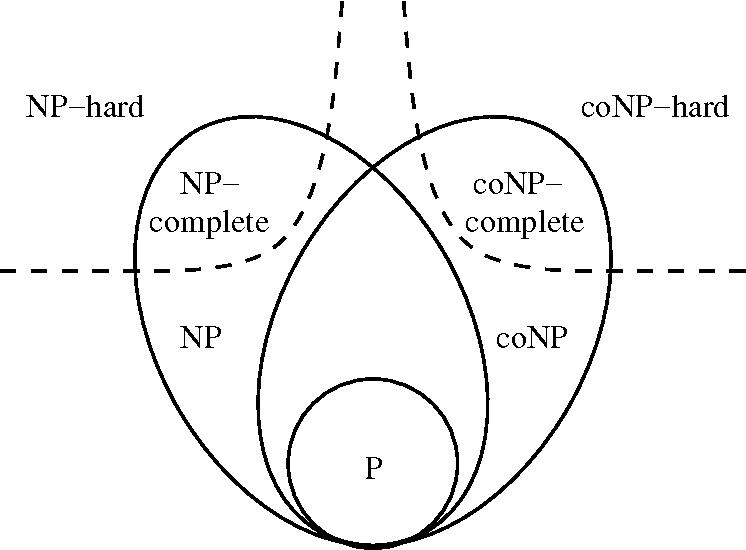
\includegraphics[width=0.9\columnwidth]{./figures/complexity_diagram.png}
    \caption{Diagramma delle classi}
    \label{fig:diagrampnpconp}
\end{figure}
